\chapter{Transferencia de calor en flujo multif\'asico tridimensional}
\label{chap:modelo3D}

La metodolog\'ia propuesta en el \chap{chap:modelo2D} demostr\'o ser una alternativa robusta para simular transferencia de calor en flujo multif\'asico bidimensional. La elecci\'on de dos \lbe{} con operador de colisi\'on MRT y definidas sobre un conjunto de velocidades D2Q9 permiti\'o alcanzar una descripci\'on macrosc\'opica precisa de las ecuaciones objetivo, sin la presencia de t\'erminos no deseados en las escalas de expansi\'on analizadas. 

Este modelo bidimensional, preciso y eficiente, puede ser aplicado en problemas reales cuya descripci\'on admite una reducci\'on de dimensiones. Sin embargo, en los problemas t\'ipicos de ebullici\'on esta aproximaci\'on muchas veces no es factible, por lo que es necesario continuar con la extensi\'on del modelo de transferencia de energ\'ia a 3 dimensiones. En el presente cap\'itulo se introduce este desarrollo para la ecuaci\'on de energ\'ia considerando un conjunto de velocidades D3Q15, y que es validado mediante los problemas de construcci\'on de Maxwell, estratificaci\'on de un fluido vdW y flujo de Stefan unidimensional.


\section{Esquema MRT para ecuaciones hidrodin\'amicas}

Los resultados obtenidos con el modelo D2Q9 motivan el desarrollo de nuevas \lbe{} basadas en la familia \pp{}. Por lo tanto, resulta natural buscar una extensi\'on de las ecuaciones a tres dimensiones, pero que tengan como base aquellos modelos desarrollados para grillas bidimensionales.

En el caso de las ecuaciones hidrodin\'amicas, el modelo de Xu y colaboradores \cite{xu_three-dimensional_2015} constituye una extensi\'on del modelo de Li \cite{li_lattice_2013} a una grilla D3Q15. Siguiendo una idea similar, este modelo introduce una \lbe{} para una funci\'on de distribuci\'on $f$ con operador de colisi\'on MRT:
\begin{equation}
	\bm{f} (\bm{x} + \bm{e}\delta_t, t+\delta_t) = \bm{M}^{-1}\left[ \bm{m} - \bm{\Lambda}(\bm{m} - \feq{m})  + \delta_t \left( \bm{I} - \dfrac{\bm{\Lambda}}{2} \bar{\bm{S}} \right) + \bm{C}\right].
	\label{eq:lbe_xu}	
\end{equation}

En este modelo, los momentos hidrodin\'amicos satisfacen:
\begin{subequations}
	\begin{equation}
		\rho = \sum_{\alpha} f_{\alpha},
	\end{equation}
	\begin{equation}
		\rho \bm{u} = \sum_{\alpha} f_{\alpha} \bm{e}_{\alpha} + \dfrac{\delta_t}{2}\bm{F},
	\end{equation}
\end{subequations}
donde $\bm{F} = \bm{F}_b + \bm{F}_i$ es la fuerza total sobre los nodos, es decir, la combinaci\'on de fuerza boyante y de interaci\'on. Usando la notaci\'on usual, $\bm{m} = \bm{Mf}$ y $\feq{m} = \bm{M}\feq{f}$ corresponden a la proyecci\'on de $\bm{f}$ y $\feq{f}$ en el espacio de momentos respectivamente, y la \edf{} queda definida en el espacio de momentos como:
\begin{equation}
	\begin{split}
		\feq{m} = \rho \left( 1, -1+|\bm{u}|^2, 1-5|\bm{u}|^2, u_x, -\dfrac{7}{3}u_x, u_y, -\dfrac{7}{3}u_y, u_z, -\dfrac{7}{3}u_z, 2u_x^2-u_y^2-u_z^2, \right.\\
		\left.\phantom{\dfrac{1}{1}} u_y^2 - u_z^2, u_xu_y, u_yu_z,u_xu_z,0 \right)^T	.
	\end{split}	
\end{equation}

Por otro lado, la matriz de colisi\'on $\bm{\Lambda}$ corresponde a una matriz diagonal con coeficientes definidos mediante:
\begin{equation}
	\bm{\Lambda} = \mbox{diag}(\tau_{\rho}^{-1}, \tau_{e}^{-1}, \tau_{\varepsilon}^{-1}, \tau_{j}^{-1}, \tau_{q}^{-1}, \tau_{j}^{-1}, \tau_{q}^{-1}, \tau_{j}^{-1}, \tau_{q}^{-1}, \tau_{\nu}^{-1}, \tau_{\nu}^{-1}, \tau_{\nu}^{-1}, \tau_{\nu}^{-1}, \tau_{\nu}^{-1}, \tau_{xyz}^{-1}),
\end{equation}
mientras que el t\'ermino de fuerza $\bm{S}$ se define en el espacio de momentos:

\begin{equation}
 \bar{\bm{S}} = 
 \left[ 
 	\begin{array}{c} 
 		0	\\
 		2 \bm{u} \cdot \bm{F} + \dfrac{6\sigma |\bm{F}|^2}{\psi^2 \delta_t (\tau_e-0.5)} \\
 		-10 \bm{u} \cdot \bm{F} \\
 		F_x \\
 		-\dfrac{7}{3}F_x \\
 		F_y \\
 		-\dfrac{7}{3}F_y \\
 		F_z \\
 		-\dfrac{7}{3}F_z \\ 		
		4u_xF_x - 2u_yF_y - 2u_zF_z \\
		2u_yF_y - 2u_zF_z \\
		u_xF_y + u_yF_x \\
		u_yF_z + u_zF_y \\
		u_xF_z + u_zF_x \\
		0
 	\end{array} 
 \right]
 \label{eq:s_xu}
\end{equation}
\FloatBarrier

De manera similar a lo que ocurre con la versi\'on de Li, el par\'ametro $\sigma$ se utiliza para ajustar parcialmente el problema de inconsistencia termodin\'amica, es decir, corregir las densidades de coexistencia recuperadas para cada fase. 

La \eq{eq:lbe_xu} incorpora un t\'ermino adicional $\bm{C}$:
\begin{equation}
 \bm{C} = 
 \left[ 
 	\begin{array}{c} 
 		0	\\
 		\dfrac{4}{5} \tau_{e}^{-1}(R_{xx} + R_{yy} + R_{zz}) \\
 		0 \\
 		0 \\
 		0 \\
 		0 \\
 		0 \\
 		0 \\
 		0 \\ 		
		-\tau_{\nu}^{-1}(2R_{xx} - R_{yy} - R_{zz}) \\
		-\tau_{\nu}^{-1}(R_{yy} - R_{zz}) \\
		-\tau_{\nu}^{-1}R_{xy} \\
		-\tau_{\nu}^{-1}R_{yz} \\
		-\tau_{\nu}^{-1}R_{xz} \\
		0
 	\end{array} 
 \right],
 \label{eq:c_xu}
\end{equation}
\FloatBarrier
donde las componentes $R_{\beta\gamma}$ corresponden al tensor $\bm{R}$ definido como:
\begin{equation}
 \bm{R} = \kappa \dfrac{G}{2} \psi(\bm{x}) \sum_{\alpha} \omega(|\bm{e}_{\alpha}|^2) \left[ \psi(\bm{x}+\bm{e}_{\alpha}) - \psi(\bm{x}) \right] \bm{e}_{\alpha}\bm{e}_{\alpha}.
	\label{eq:R_xu}
\end{equation}

En este caso, puede demostrarse que la incorporaci\'on del t\'ermino $\bm{C}$ permite  ajustar la tensi\'on superficial recuperada ($\sigma_s$) mediante la constante $\kappa$ de la \eq{eq:R_xu}. El an\'alisis de Chapman-Enskog de este esquema muestra que es posible recuperar las siguientes ecuaci\'ones de conservaci\'on de masa e impulso lineal:
\begin{subequations}
	\begin{equation}
		\dfrac{\partial \rho}{\partial t} + \nabla \cdot (\rho \bm{u}) = 0,
	\end{equation}
	\begin{equation}
		\begin{aligned}
		\dfrac{\partial(\rho\bm{u})}{\partial t} + \nabla \cdot (\rho \bm{u} \bm{u})  = &-\nabla \cdot(\rho c_s^2)\bm{I} + \nabla \cdot \bm{\Pi} + \bm{F} - 2G^2 c^4 \sigma \nabla \cdot (|\nabla \psi|^2 \bm{I}) \\
		& -\nabla \cdot \left[ \kappa \dfrac{Gc^4}{6} (\psi \nabla^2 \psi \bm{I} - \psi \nabla \nabla \psi) \right],
		\end{aligned}
	\end{equation}
	\label{eq:xu_macro}
\end{subequations}
donde el tensor de tensiones $\bm{\Pi}$ se define como:
\begin{equation}
	\bm{\Pi} = \rho \nu \left[ \nabla \bm{u} + (\nabla \bm{u})^T \right] + \rho \left( \xi - \dfrac{2}{3}\nu \right) (\nabla \cdot \bm{u})\bm{I},
\end{equation}
y las viscosidades cinem\'atica y de volumen corresponden a:
\begin{subequations}
	\begin{equation}
		\nu = \dfrac{1}{3} \left( \tau_{\nu} - \dfrac{1}{2}\right) \delta_t,
	\end{equation}
	\begin{equation}
		\xi = \dfrac{2}{9} \left( \tau_{e} - \dfrac{1}{2}\right) \delta_t.
	\end{equation}	
\end{subequations}

Como puede observarse, la \eq{eq:xu_macro} es similar al conjunto de ecuaciones recuperadas por el modelo bidimensional de Li (\eq{eq:li_macro}), salvo por la presencia de t\'erminos dependientes de $\kappa$ que contribuyen a la recuperaci\'on de tensi\'on superficial en la interfase. En particular, si se utiliza la expresi\'on discreta para el tensor de presiones introducida por Shan \cite{shan_pressure_2008}, es posible ver que la forma macrosc\'opica de este tensor finalmente resulta:
\begin{equation}
	\bm{P} = \left[ \rho c_s^2 + \dfrac{G c^2}{2} \psi^2 + \dfrac{G c^4}{12} (1+2\kappa) \psi \nabla^2 \psi + 2 \sigma G^2 c^4 |\nabla \psi|^2\right] \bm{I} + \dfrac{G c^4}{6} (1-\kappa) \psi \nabla \nabla \psi.
	\label{eq:PTens_Xu}
\end{equation}


\subsection{Condiciones de contorno}
\label{sec:nebb_d3q15}

La selecci\'on de condiciones de contorno para el modelo tridimensional sigue una estrategia similar a la utilizada con la versi\'on D2Q9, donde la \lbe{} hidrodin\'amica puede resolverse junto con la condici\'on de \emph{bounce-back} de las componentes de no equilibrio en aquellas fronteras que presenten un valor de velocidad arbitrario.

La condici\'on de NEBB s\'olo puede aplicarse sobre superficies planas cuya normal se encuentra alineada con alguno de los ejes principales de coordenadas. Por lo tanto, s\'olo es necesario desarrollar expl\'icitamente las componentes desconocidas para una normal, y derivar las restantes simplemente por transformaci\'on de coordenadas. A modo de ejemplo, en la \fig{fig:d3q15_normal_plane} se observa un plano con normal saliente en la direcci\'on $(-1,0,0)$, junto con el conjunto de velocidades D3Q15. En este caso, despu\'es del paso de advecci\'on es necesario determinar las componentes $f_{\alpha}$ con $\alpha=1,7,9,11,13$. 
\begin{figure}[ht]
	\centering
	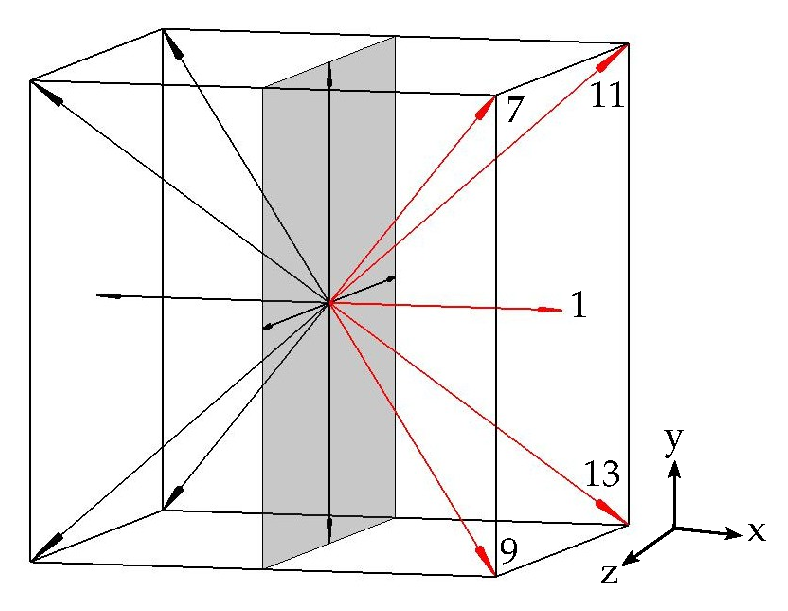
\includegraphics[width=0.75\textwidth]{NEBB_D3Q15}
	\caption{Plano con normal saliente en $(-1,0,0)$, sobre un conjunto de velocidades D3Q15. En color rojo se indican las componentes que deben corregirse despu\'es del paso de advecci\'on.}
	\label{fig:d3q15_normal_plane}
\end{figure}

Si s\'olo se aplica NEBB a la componente normal a la frontera ($\alpha=1$) quedan 4 componentes a determinar, junto con la densidad sobre la pared. Sin embargo, como s\'olo se tienen 4 momentos macrosc\'opicos ($\rho$, $\rho u_x$, $\rho u_y$, $\rho u_z$) sigue siendo necesario incorporar una ecuaci\'on adicional. Siguiendo la propuesta de Zou y He \cite{zou_pressure_1997} podemos utilizar NEBB para todas las componentes desconocidas y aplicar correctores de impulso, es decir 
\begin{equation}
	\begin{aligned}
		f_{\alpha} &= f_{\bar{\alpha}} + f_{\alpha}^{eq} - f_{\bar{\alpha}}^{eq}, \qquad  \alpha=1 \\
		f_{\alpha} &= f_{\bar{\alpha}} + f_{\alpha}^{eq} - f_{\bar{\alpha}}^{eq} + k_{\Delta} \bm{e}_{\alpha} \cdot \Delta,    \qquad  \alpha=7,9,11,13,
	\end{aligned}
\end{equation}
donde $\Delta=(\delta_x,\delta_y,\delta_z)$ es el corrector de impulso y $k_{\Delta}$ corresponde a una constante arbitraria. Con esta estrategia se hace uso de las componentes en las direcciones conocidas, y el problema se reduce a calcular simplemente las 3 componentes de $\Delta$ y la densidad sobre la pared $\rho_w$:
\begin{subequations}
	\begin{equation}
		f_1 = f_2 + \dfrac{2}{3}\rho_w u_{w_x},
	\end{equation}
	\begin{equation}
		f_7 = f_{14} + \dfrac{1}{12}\rho_w (u_{w_x} + u_{w_y} + u_{w_z}) + k (\delta_x+\delta_y+\delta_z),
	\end{equation}
	\begin{equation}
		f_9 = f_{12} + \dfrac{1}{12}\rho_w (u_{w_x} - u_{w_y} + u_{w_z}) + k (\delta_x-\delta_y+\delta_z),
	\end{equation}	
	\begin{equation}
		f_{11} = f_{10} + \dfrac{1}{12}\rho_w (u_{w_x} + u_{w_y} - u_{w_z}) + k (\delta_x+\delta_y-\delta_z),
	\end{equation}
	\begin{equation}
		f_{13} = f_{8} + \dfrac{1}{12}\rho_w (u_{w_x} - u_{w_y} - u_{w_z}) + k (\delta_x-\delta_y-\delta_z).
	\end{equation}
	\label{eq:NEBB_unk_3d}	
\end{subequations}

Las componentes del corrector de impulso pueden obtenerse a partir de los diferentes momentos macrosc\'opicos de $f$ sobre la frontera. Por ejemplo, para $\rho u_{w_x}$ se tiene:
\begin{equation}
	\rho u_{w_x} = \sum_{\alpha} e_{\alpha_x}f_{\alpha} = -f_2 - f_8 - f_{10} - f_{12}- f_{14} + f_1 + f_7 + f_9 + f_{11} + f_{13} + \dfrac{\delta_t}{2} F_x,
\end{equation} 
y usando las definiciones de la \eq{eq:NEBB_unk_3d} para reescribir $\rho u_{w_x}$ puede obtenerse:
\begin{equation}
	\delta_x=-\dfrac{\delta_t}{8k}F_x.
\end{equation}

Esta idea puede usarse para determinar los correctores restantes a partir de la definici\'on de $\rho u_{w_y}$ y $\rho u_{w_z}$:
\begin{equation}
	\delta_y = \dfrac{1}{k}\left[ -\dfrac{1}{4}(f_3 - f_4) + \dfrac{1}{6}\rho_w u_{w_y} - \dfrac{\delta_t}{8}F_y \right],
\end{equation}
\begin{equation}
	\delta_y = \dfrac{1}{k}\left[ -\dfrac{1}{4}(f_5 - f_6) + \dfrac{1}{6}\rho_w u_{w_z} - \dfrac{\delta_t}{8}F_z \right].
\end{equation}

S\'olo resta encontrar el valor de densidad sobre la frontera. Usando el momento de orden 0 de $f$ y la \eq{eq:NEBB_unk_3d} para las componentes desconocidas resulta:
\begin{equation}
	\rho_w = \dfrac{1}{1-u_{w_x}} \left[   f_0 + f_3 + f_4 + f_5 + f_6 + 2(f_2 + f_8 + f_{10} + f_{12} + f_{14}) + 4k\delta_x \right].
\end{equation}





\section{Esquema MRT para ecuaci\'on de energ\'ia}

En el \chap{chap:modelo2D} se mostr\'o que es posible acoplar una segunda \lbe{} a un esquema de la famila \pp{}, y de esta forma poder simular transferencia de calor y cambio de fase en flujos multif\'asicos. En particular, si se elige adecuadamente a la \edf{}, matriz de relajaci\'on y t\'ermino fuente, se mostr\'o formalmente que es posible recuperar una soluci\'on macrosc\'opica dada por la \eq{eq:markus}, sin t\'erminos adicionales hasta la escala de expansi\'on analizada. Por otro lado, la metodolog\'ia empleada demostr\'o proveer un camino consistente para el desarrollo de nuevas \lbe{} para la resoluci\'on de ecuaciones de energ\'ia similares, eficientes y flexibles en la reproducci\'on de las propiedades macrosc\'opicas relevantes.

Estas caracter\'isticas positivas observadas en el modelo bidimensional motivan la continuaci\'on de esta l\'inea de desarrollo. De esta manera, la nueva propuesta consiste en emplear una \lbe{} con operador de colisi\'on MRT sobre un conjunto de velocidades D3Q15:
\begin{subequations}
	\begin{equation}
		\bm{g}(\bm{x} + \bm{e} \delta_t, t+\delta_t) = \bm{M}^{-1} \left[ \bm{n} - \bm{Q}(\bm{n} - \feq{n}) + \delta_t \left( \bm{I}-\dfrac{\bm{Q}}{2}\right) \bm{\Gamma}\right],
		\label{eq:g_model_3d}
	\end{equation}	
	\begin{equation}
		T = \sum_{\alpha} g_{\alpha} + \dfrac{\delta_t}{2} \Gamma_0,
	\end{equation}
\end{subequations}
donde las variables del miembro derecho se encuentran definidas en $(\bm{x},t)$. En este caso, $\bm{n} = \bm{Mg}$,  $\feq{n} = \bm{M}\feq{g}$, y $\bm{\Gamma}$ corresponde a un t\'ermino de fuente definido en el espacio de momentos. 

Continuando con las ideas desarrolladas en el \chap{chap:modelo2D}, es posible introducir una distribuci\'on de equilibrio y el t\'ermino de fuente directamente en el espacio de momentos:
\begin{equation}
	\feq{n} = T ( 1, \alpha_1, \alpha_2, \alpha_3u_x, \alpha_4u_x, \alpha_5u_y, \alpha_6u_y, \alpha_7u_z, \alpha_8u_z,0,0,0,0,0,0)^T,
\end{equation}
\begin{equation}
	\bm{\Gamma} = (s,0,0,0,0,0,0,0,0,0,0,0,0,0,0)^T.	
\end{equation}

Por otro lado, es necesario incluir una matriz de relajaci\'on con coeficientes no nulos en la diagonal, que en este caso corresponde a los elementos $q_{34}$, $q_{56}$ y $q_{78}$.
%\setcounter{MaxMatrixCols}{15}
%\begin{equation}
%	\bm{Q}=
%	\begin{bmatrix}
%	q_0 & 0 & 0 & 0 & 0 & 0 & 0 & 0 & 0 & 0 & 0 & 0 & 0 & 0 & 0 \\
%	0 & q_1 & 0 & 0 & 0 & 0 & 0 & 0 & 0 & 0 & 0 & 0 & 0 & 0 & 0 \\
%	0 & 0 & q_2 & 0 & 0 & 0 & 0 & 0 & 0 & 0 & 0 & 0 & 0 & 0 & 0 \\
%	0 & 0 & 0 & q_3 & q_{34} & 0 & 0 & 0 & 0 & 0 & 0 & 0 & 0 & 0 & 0 \\
%	0 & 0 & 0 & 0 & q_4 & 0 & 0 & 0 & 0 & 0 & 0 & 0 & 0 & 0 & 0 \\
%	0 & 0 & 0 & 0 & 0 & q_5 & q_{56} & 0 & 0 & 0 & 0 & 0 & 0 & 0 & 0 \\
%	0 & 0 & 0 & 0 & 0 & 0 & q_6 & 0 & 0 & 0 & 0 & 0 & 0 & 0 & 0 \\
%	0 & 0 & 0 & 0 & 0 & 0 & 0 & q_7 & q_{78} & 0 & 0 & 0 & 0 & 0 & 0 \\
%	0 & 0 & 0 & 0 & 0 & 0 & 0 & 0 & q_8 & 0 & 0 & 0 & 0 & 0 & 0 \\
%	0 & 0 & 0 & 0 & 0 & 0 & 0 & 0 & 0 & q_{9} & 0 & 0 & 0 & 0 & 0 \\
%	0 & 0 & 0 & 0 & 0 & 0 & 0 & 0 & 0 & 0 & q_{10} & 0 & 0 & 0 & 0 \\
%	0 & 0 & 0 & 0 & 0 & 0 & 0 & 0 & 0 & 0 & 0 & q_{11} & 0 & 0 & 0 \\
%	0 & 0 & 0 & 0 & 0 & 0 & 0 & 0 & 0 & 0 & 0 & 0 & q_{12} & 0 & 0 \\
%	0 & 0 & 0 & 0 & 0 & 0 & 0 & 0 & 0 & 0 & 0 & 0 & 0 & q_{13} & 0 \\
%	0 & 0 & 0 & 0 & 0 & 0 & 0 & 0 & 0 & 0 & 0 & 0 & 0 & 0 & q_{14}
%	\end{bmatrix}
%\end{equation}

La expansi\'on en serie de Taylor de la \eq{eq:g_model_3d} lleva a una expresi\'on similar a la \eq{eq:model_2d_momento}:
\begin{equation}
	\dcm \bm{n} + \dfrac{\delta_t}{2} \dcm^2 \bm{n} = -\dfrac{1}{\delta_t}\bm{Q}(\bm{n} - \feq{n}) + \delta_t \left( \bm{I}-\dfrac{\bm{Q}}{2}\right) \bm{\Gamma},
	\label{eq:model_3d_momento}
\end{equation}
y, por lo tanto, a la misma descomposici\'on en escalas de $\varepsilon$ dentro del an\'alisis de Chapman-Enskog. En particular, si se aplica la expansi\'on dada por:
\begin{subequations}
	\begin{equation}
		\bm{n} = \bc{n}{0} + \varepsilon \bc{n}{1} + \varepsilon^2 \bc{n}{2} + \cdots = \sum_{k=0}^{\infty} \varepsilon^k \bc{n}{k},
	\end{equation}
	\begin{equation}
		\dfrac{\partial}{\partial t} = \varepsilon \dfrac{\partial}{\partial t_1} + 	\varepsilon^2 \dfrac{\partial}{\partial t_2},
	\end{equation}
	\begin{equation}
		\dfrac{\partial}{\partial x_{\beta}} = \varepsilon \dfrac{\partial}{\partial x_{\beta_1}},
	\end{equation}
	\begin{equation}
		\bm{\Gamma} = \varepsilon \bc{\Gamma}{1},
	\end{equation}
	\label{eq:escalas_che_3D}
\end{subequations}
entonces puede descomponerse a la \eq{eq:model_3d_momento} en ecuaciones individuales para cada potencia de $\varepsilon$:
\begin{subequations}
	\begin{align}
		\varepsilon^0: & \, \bc{n}{0} = \feq{n} \label{eq:eps_0_3d}\\
		\varepsilon^1: & \, \dcmuno \bc{n}{0} - \bc{\Gamma}{1} = -\dfrac{1}{\delta_t} \bm{Q} \left( \bc{n}{1} + \dfrac{\delta_t}{2} \bc{\Gamma}{1} \right)  \label{eq:eps_1_3d}\\
		\varepsilon^2: & \, \dcmuno \left( \bm{I}-\dfrac{\bm{Q}}{2}\right) \left( \bc{n}{1} + \dfrac{\delta_t}{2} \bc{\Gamma}{1} \right) + \dfrac{\partial \bc{n}{0}}{\partial t_2}  =  -\dfrac{1}{\delta_t} \bm{Q} \bc{n}{2}. \label{eq:eps_2_3d}
	\end{align}
\end{subequations}

La definici\'on de las matrices $\hat{\bm{E}}_{\beta}$ es similar a la del caso bidimensional, por lo que corresponden a $\hat{\bm{E}}_{\beta} = \bm{M} \bm{E}_{\beta} \bm{M}^{-1}$, con $\bm{E}_{\beta} = diag(e_{0\beta} \cdots e_{q-1\beta})$. En una grilla D3Q15, donde $\beta=x,y,z$ y se tiene un conjunto diferente de velocidades de grilla, estas matrices resultan:
\setcounter{MaxMatrixCols}{15}
\begin{equation}
	\hat{\bm{E}}_{x}=
	\begin{bmatrix}
	0 & 0 & 0 & 1 & 0 & 0 & 0 & 0 & 0 & 0 & 0 & 0 & 0 & 0 & 0 \\
	0 & 0 & 0 & 3/5 & 2/5 & 0 & 0 & 0 & 0 & 0 & 0 & 0 & 0 & 0 & 0 \\
	0 & 0 & 0 & 0 & 1 & 0 & 0 & 0 & 0 & 0 & 0 & 0 & 0 & 0 & 0 \\
	2/3 & 1/3 & 0 & 0 & 0 & 0 & 0 & 0 & 0 & 1/3 & 0 & 0 & 0 & 0 & 0 \\
	0 & 8/9 & 1/9 & 0 & 0 & 0 & 0 & 0 & 0 & -4/3 & 0 & 0 & 0 & 0 & 0 \\
	0 & 0 & 0 & 0 & 0 & 0 & 0 & 0 & 0 & 0 & 0 & 1 & 0 & 0 & 0 \\
	0 & 0 & 0 & 0 & 0 & 0 & 0 & 0 & 0 & 0 & 0 & 1 & 0 & 0 & 0 \\
	0 & 0 & 0 & 0 & 0 & 0 & 0 & 0 & 0 & 0 & 0 & 0 & 0 & 1 & 0 \\
	0 & 0 & 0 & 0 & 0 & 0 & 0 & 0 & 0 & 0 & 0 & 0 & 0 & 1 & 0 \\
	0 & 0 & 0 & 2/5 & -2/5 & 0 & 0 & 0 & 0 & 0 & 0 & 0 & 0 & 0 & 0 \\
	0 & 0 & 0 & 0 & 0 & 0 & 0 & 0 & 0 & 0 & 0 & 0 & 0 & 0 & 0 \\
	0 & 0 & 0 & 0 & 0 & 4/5 & 1/5 & 0 & 0 & 0 & 0 & 0 & 0 & 0 & 0 \\
	0 & 0 & 0 & 0 & 0 & 0 & 0 & 0 & 0 & 0 & 0 & 0 & 0 & 0 & 1 \\
	0 & 0 & 0 & 0 & 0 & 0 & 0 & 4/5 & 1/5 & 0 & 0 & 0 & 0 & 0 & 0 \\
	0 & 0 & 0 & 0 & 0 & 0 & 0 & 0 & 0 & 0 & 0 & 0 & 1 & 0 & 0 \\
	\end{bmatrix},
\end{equation} 

\begin{equation}
	\hat{\bm{E}}_{y}=
	\begin{bmatrix}
	0 & 0 & 0 & 0 & 1 & 0 & 0 & 0 & 0 & 0 & 0 & 0 & 0 & 0 & 0 \\
	0 & 0 & 0 & 0 & 3/5 & 2/5 & 0 & 0 & 0 & 0 & 0 & 0 & 0 & 0 & 0 \\
	0 & 0 & 0 & 0 & 0 & 0 & 1 & 0 & 0 & 0 & 0 & 0 & 0 & 0 & 0 \\
	0 & 0 & 0 & 0 & 0 & 0 & 0 & 0 & 0 & 0 & 0 & 1 & 0 & 0 & 0 \\
	0 & 0 & 0 & 0 & 0 & 0 & 0 & 0 & 0 & 0 & 0 & 1 & 0 & 0 & 0 \\
	2/3 & 1/3 & 0 & 0 & 0 & 0 & 0 & 0 & 0 & -1/6 & 1/2 & 0 & 0 & 0 & 0 \\
	0 & 8/9 & 1/9 & 0 & 0 & 0 & 0 & 0 & 0 & 2/3 & -2 & 0 & 0 & 0 & 0 \\
	0 & 0 & 0 & 0 & 0 & 0 & 0 & 0 & 0 & 0 & 0 & 0 & 0 & 1 & 0 \\
	0 & 0 & 0 & 0 & 0 & 0 & 0 & 0 & 0 & 0 & 0 & 0 & 0 & 1 & 0 \\
	0 & 0 & 0 & 0 & -1/5 & 1/5 & 0 & 0 & 0 & 0 & 0 & 0 & 0 & 0 & 0 \\
	0 & 0 & 0 & 0 & 1/5 & -1/5 & 0 & 0 & 0 & 0 & 0 & 0 & 0 & 0 & 0 \\
	0 & 0 & 0 & 4/5 & 1/5 & 0 & 0 & 0 & 0 & 0 & 0 & 0 & 0 & 0 & 0 \\
	0 & 0 & 0 & 0 & 0 & 0 & 0 & 4/5 & 1/5 & 0 & 0 & 0 & 0 & 0 & 0 \\
	0 & 0 & 0 & 0 & 0 & 0 & 0 & 0 & 0 & 0 & 0 & 0 & 0 & 0 & 1 \\
	0 & 0 & 0 & 0 & 0 & 0 & 0 & 0 & 0 & 0 & 0 & 0 & 0 & 1 & 0 \\
	\end{bmatrix}
\end{equation} 

y 

\begin{equation}
	\hat{\bm{E}}_{z}=
	\begin{bmatrix}
	0 & 0 & 0 & 0 & 0 & 0 & 0 & 1 & 0 & 0 & 0 & 0 & 0 & 0 & 0 \\
	0 & 0 & 0 & 0 & 0 & 0 & 0 & 3/5 & 2/5 & 0 & 0 & 0 & 0 & 0 & 0 \\
	0 & 0 & 0 & 0 & 0 & 0 & 0 & 0 & 1 & 0 & 0 & 0 & 0 & 0 & 0 \\
	0 & 0 & 0 & 0 & 0 & 0 & 0 & 0 & 0 & 0 & 0 & 0 & 0 & 1 & 0 \\
	0 & 0 & 0 & 0 & 0 & 0 & 0 & 0 & 0 & 0 & 0 & 0 & 0 & 1 & 0 \\
	0 & 0 & 0 & 0 & 0 & 0 & 0 & 0 & 0 & 0 & 0 & 0 & 1 & 0 & 0 \\
	0 & 0 & 0 & 0 & 0 & 0 & 0 & 0 & 0 & 0 & 0 & 0 & 1 & 0 & 0 \\
	2/3 & 1/3 & 0 & 0 & 0 & 0 & 0 & 0 & 0 & -1/6 & -1/2 & 0 & 0 & 0 & 0 \\
	0 & 8/9 & 1/9 & 0 & 0 & 0 & 0 & 0 & 0 & 2/3 & 2 & 0 & 0 & 0 & 0 \\
	0 & 0 & 0 & 0 & 0 & 0 & 0 & -1/5 & 1/5 & 0 & 0 & 0 & 0 & 0 & 0 \\
	0 & 0 & 0 & 0 & 0 & 0 & 0 & -1/5 & 1/5 & 0 & 0 & 0 & 0 & 0 & 0 \\
	0 & 0 & 0 & 0 & 0 & 0 & 0 & 0 & 0 & 0 & 0 & 0 & 0 & 0 & 1 \\
	0 & 0 & 0 & 0 & 0 & 4/5 & 1/5 & 0 & 0 & 0 & 0 & 0 & 0 & 0 & 0 \\
	0 & 0 & 0 & 4/5 & 1/5 & 0 & 0 & 0 & 0 & 0 & 0 & 0 & 0 & 0 & 0 \\
	0 & 0 & 0 & 0 & 0 & 0 & 0 & 0 & 0 & 0 & 0 & 1 & 0 & 0 & 0 \\
	\end{bmatrix}.
\end{equation} 

En definitiva, el desarrollo de Taylor y la expansi\'on de Chapman-Enskog empleada en el \chap{chap:modelo2D} son aplicables al nuevo conjunto de velocidades, aunque naturalmente deben considerarse nuevas estructuras para $\feq{n}$, $\bm{Q}$ y $\hat{\bm{E}}_{\beta}$. 

La ecuaci\'on recuperada en la escala $\varepsilon^1$ puede obtenerse a partir de la primera componente de la \eq{eq:eps_1_3d}:
\begin{equation}
	\dfrac{\partial \nce{0}{0}}{\partial t_1} 
	+ \dfrac{\partial \nce{3}{0}}{\partial x_1}
	+ \dfrac{\partial \nce{5}{0}}{\partial y_1}
	+ \dfrac{\partial \nce{7}{0}}{\partial z_1}		
	- \Gamma_0^{(1)}
	= - \dfrac{1}{\delta_t} q_0 \left( \nce{0}{1} + \dfrac{\delta_t}{2} \Gamma_0^{(1)} \right).
	\label{eq:eps1_comp_3d}
\end{equation}

Usando la descomposici\'on de escalas de la \eq{eq:ncero_che}, es decir:
\begin{equation}
	\begin{aligned}
		\varepsilon^0: && \nce{0}{0} = n_0^{eq} \\
		\varepsilon^1: && \nce{0}{1} + \dfrac{\delta_t}{2} \Gamma_0^{(1)} = 0\\
		\varepsilon^2: && \nce{0}{2} = 0 \\
		&\vdots& \\
		\varepsilon^k: && \nce{0}{k} = 0 \quad \forall \, k > 2,
	\end{aligned}
\end{equation}
entonces puede reescribirse a la \eq{eq:eps1_comp_3d} como:
\begin{equation}
	\dfrac{\partial T}{\partial t_1} 
	+ \dfrac{\partial (\alpha_3 T u_x)}{\partial x_1}
	+ \dfrac{\partial (\alpha_5 T u_y)}{\partial y_1}
	+ \dfrac{\partial (\alpha_7 T u_z)}{\partial z_1}		
	- \Gamma_0^{(1)} = 0.
\end{equation}

Por lo tanto, si $\alpha_3 = \alpha_5 = \alpha_7 = 1$, se obtiene una ecuaci\'on recuperada en la escala $\varepsilon^1$:
\begin{equation}
	\dfrac{\partial T}{\partial t_1}  + \nabla_1 \cdot (T \bm{u}) - \Gamma_0^{(1)} = 0.
	\label{eq:eps1_T_3d}
\end{equation}

Por otro lado, la ecuaci\'on recuperada en la escala $\varepsilon^2$ puede obtenerse a partir de la primera componente de la \eq{eq:eps_2_3d}:
\begin{equation}
	\dfrac{\partial \nce{0}{0}}{\partial t_2} 
	+ \dfrac{\partial \nces{0}{1}}{\partial t_1} 	
	+ \dfrac{\partial \nces{3}{0}}{\partial x_1}
	+ \dfrac{\partial \nces{5}{0}}{\partial y_1}
	+ \dfrac{\partial \nces{7}{0}}{\partial z_1}		
	= - \dfrac{1}{\delta_t} q_0 \nce{0}{2} = 0,
	\label{eq:eps2_comp_3d}
\end{equation}
donde se definieron las componentes
\begin{subequations}
	\begin{equation}
		\nces{0}{1} = \left( 1 - \dfrac{q_0}{2} \right) \left( \nce{0}{1} + \dfrac{\delta_t}{2} \Gamma_0^{(1)} \right) = 0,
	\end{equation}
	\begin{equation}
		\nces{3}{1} = \left( 1 - \dfrac{q_3}{2} \right) \nce{3}{1} + \dfrac{q_{34}}{2}\nce{4}{1},
		\label{eq:n3star_3d}
	\end{equation}	
	\begin{equation}
		\nces{5}{1} = \left( 1 - \dfrac{q_5}{2} \right) \nce{5}{1} + \dfrac{q_{56}}{2}\nce{6}{1},
	\end{equation}		
	\begin{equation}
		\nces{7}{1} = \left( 1 - \dfrac{q_7}{2} \right) \nce{7}{1} + \dfrac{q_{78}}{2}\nce{8}{1}.
	\end{equation}			
\end{subequations}

De esta manera, se necesitan ecuaciones que permitan expresar a $\nce{3}{1}$, $\nce{4}{1}$, $\nce{5}{1}$, $\nce{6}{1}$, $\nce{7}{1}$ y $\nce{8}{1}$ en funci\'on de las variables macrosc\'opicas, es decir $\rho$, $\bm{u}$ y $T$. Nuevamente, esta descripci\'on puede obtenerse a partir de las componentes relevantes de la \eq{eq:eps_1_3d}, como se ejemplifica para $\nce{3}{1}$:
\begin{equation}
	\dfrac{\partial \nce{3}{0}}{\partial t_1} 
	+ \dfrac{2}{3} \dfrac{\partial \nce{0}{0}}{\partial x_1}
	+ \dfrac{1}{3} \dfrac{\partial \nce{1}{0}}{\partial x_1}	
	+ \dfrac{1}{3} \dfrac{\partial \nce{9}{0}}{\partial x_1}	
	+ \dfrac{\partial \nce{11}{0}}{\partial y_1}	
	+ \dfrac{\partial \nce{13}{0}}{\partial z_1}	
	= -\dfrac{1}{\delta_t} q_3 \nce{3}{1} -\dfrac{1}{\delta_t} q_{34} \nce{4}{1}
\end{equation}
\begin{equation}
	\dfrac{\partial (Tu_x)}{\partial t_1} 
	+ \dfrac{\partial}{\partial x_1} \left( \dfrac{2+\alpha_1}{3}T \right)
	= -\dfrac{1}{\delta_t} q_3 \nce{3}{1} -\dfrac{1}{\delta_t} q_{34} \nce{4}{1}
	\label{eq:n3_eps1_3d}
\end{equation}

Por otro lado, para $\nce{4}{1}$ se tiene:
\begin{equation}
	\dfrac{\partial \nce{4}{0}}{\partial t_1} 
	+ \dfrac{8}{9} \dfrac{\partial \nce{1}{0}}{\partial x_1}
	+ \dfrac{1}{9} \dfrac{\partial \nce{2}{0}}{\partial x_1}	
	- \dfrac{4}{3} \dfrac{\partial \nce{9}{0}}{\partial x_1}	
	+ \dfrac{\partial \nce{11}{0}}{\partial y_1}	
	+ \dfrac{\partial \nce{13}{0}}{\partial z_1}	
	= -\dfrac{1}{\delta_t} q_4 \nce{4}{1},
\end{equation}
y si $\alpha_4=-1$ resulta:
\begin{equation}
	-\dfrac{\partial (Tu_x)}{\partial t_1} 
	+ \dfrac{\partial}{\partial x_1} \left( \dfrac{8\alpha_1+\alpha_2}{9}T \right)
	=-\dfrac{1}{\delta_t} q_4 \nce{4}{1}
	\label{eq:n4_eps1_3d}
\end{equation}

Si se despejan $\nce{3}{1}$ y $\nce{4}{1}$ de las \eqs{eq:n3_eps1_3d}{eq:n4_eps1_3d}, entonces puede reescribirse a la \eq{eq:n3star_3d} como:
\begin{equation}
	\begin{aligned}
	    \nces{3}{1} = &- \delta_t \left( \dfrac{1}{q_3} - \dfrac{1}{2} \right) \left[ \dfrac{\partial (Tu_x)}{\partial t_1} + \dfrac{\partial}{\partial x_1} \left( \dfrac{2+\alpha_1}{3}T \right) \right] \\
	    &+ \delta_t \dfrac{q_{34}}{q_3 q_4} \left[ -\dfrac{\partial (Tu_x)}{\partial t_1} + \dfrac{\partial}{\partial x_1} \left( \dfrac{8\alpha_1+\alpha_2}{9}T \right) \right].
	\end{aligned}
	\label{eq:n3star_final_3d}
\end{equation}

Por lo tanto, es posible ver que si el coeficiente de relajaci\'on $q_{34}$ satisface
\begin{equation}
	q_{34} = q_4 \left( \dfrac{q_3}{2} - 1 \right),
\end{equation}
entonces se anulan las derivadas temporales de $\nces{3}{1}$ y la \eq{eq:n3star_final_3d} finalmente resulta:
\begin{equation}
	\nces{3}{1} = -\delta_t \left( \dfrac{1}{q_3} - \dfrac{1}{2} \right) \dfrac{\partial}{\partial x_1} \left( \dfrac{6 + 11\alpha_1+\alpha_2}{9}T \right).
	\label{eq:n3star_macro 3d}
\end{equation}

Este mismo procedimiento puede utilizarse para reescribir a $\nces{5}{1}$ y $\nces{7}{1}$. En particular, si $\alpha_6 = \alpha_8 = -1$, y definiendo los coeficientes de relajaci\'on $q_{56}$ y $q_{78}$ como:
\begin{equation}
	q_{56} = q_6 \left( \dfrac{q_{5}}{2} - 1 \right),
\end{equation}
\begin{equation}
	q_{78} = q_8 \left( \dfrac{q_{7}}{2} - 1 \right),
\end{equation}
entonces se tiene:
\begin{equation}
	\nces{5}{1} = -\delta_t \left( \dfrac{1}{q_5} - \dfrac{1}{2} \right) \dfrac{\partial}{\partial y_1} \left( \dfrac{6 + 11\alpha_1+\alpha_2}{9}T \right),
	\label{eq:n5star_macro 3d}
\end{equation}
\begin{equation}
	\nces{7}{1} = -\delta_t \left( \dfrac{1}{q_7} - \dfrac{1}{2} \right) \dfrac{\partial}{\partial z_1} \left( \dfrac{6 + 11\alpha_1+\alpha_2}{9}T \right).
	\label{eq:n7star_macro 3d}
\end{equation}

Finalmente, la ecuaci\'on macrosc\'opica recuperada en escala $\varepsilon^2$ (\eq{eq:eps2_comp_3d}) puede reescribirse en funci\'on de las variables macrosc\'opicas usando las \eqto{eq:n3star_macro 3d}{eq:n7star_macro 3d}, e imponiendo la restricci\'on $q_3=q_5=q_7=q_{\chi}$:
\begin{equation}
	\begin{aligned}
		\dfrac{\partial T}{\partial t_2} 
		&- \dfrac{\partial}{\partial x_1}\left[ \delta_t \left( \dfrac{1}{q_{\chi}} - \dfrac{1}{2} \right) \dfrac{\partial}{\partial x_1} \left( \dfrac{6 + 11\alpha_1+\alpha_2}{9}T \right) \right] \\
		&- \dfrac{\partial}{\partial y_1}\left[ \delta_t \left( \dfrac{1}{q_{\chi}} - \dfrac{1}{2} \right) \dfrac{\partial}{\partial y_1} \left( \dfrac{6 + 11\alpha_1+\alpha_2}{9}T \right) \right] \\
		&- \dfrac{\partial}{\partial z_1}\left[ \delta_t \left( \dfrac{1}{q_{\chi}} - \dfrac{1}{2} \right) \dfrac{\partial}{\partial z_1} \left( \dfrac{6 + 11\alpha_1+\alpha_2}{9}T \right) \right] = 0,
	\end{aligned}
\end{equation}

\begin{equation}
	\dfrac{\partial T}{\partial t_2} - \nabla_1 \cdot \left[ \delta_t \left( \dfrac{1}{q_{\chi}} - \dfrac{1}{2} \right) \left( \dfrac{6 + 11\alpha_1+\alpha_2}{9} \right) \nabla_1 T \right] = 0,
	\label{eq:eps2_T_3d}
\end{equation}

El an\'alisis de la expansi\'on de Chapman-Enskog finaliza con la combinaci\'on de las ecuaciones macrosc\'opicas obtenidas para cada escala. Por lo tanto, multiplicando por $\varepsilon$ a la \eq{eq:eps1_T_3d}, por $\varepsilon^2$ a la \eq{eq:eps2_T_3d} y sum\'andolas, se tiene:
\begin{equation}
	\varepsilon \dfrac{\partial T}{\partial t_1} + \varepsilon^2 \dfrac{\partial T}{\partial t_2} + \varepsilon \nabla_1 \cdot (T\bm{u}) - \varepsilon^2 \nabla_1 \cdot (\chi \nabla T) - \varepsilon \Gamma_0^{(1)} = 0,
\end{equation}
donde se define a la difusividad t\'ermica $\chi$ como:
\begin{equation}
	\chi = \delta_t \left( \dfrac{1}{q_{\chi}} - \dfrac{1}{2} \right) \left( \dfrac{6 + 11\alpha_1+\alpha_2}{9} \right).
	\label{eq:modelo_3d_chi}
\end{equation}

Usando la expansi\'on de escalas dada por la \eq{eq:escalas_che_3D}, la ecuaci\'on macroc\'opica recuperada finalmente resulta:
\begin{equation}
	\dfrac{\partial T}{\partial t} + \nabla \cdot (T\bm{u}) = \nabla \cdot (\chi \nabla T) + s.
	\label{eq:T_3d}
\end{equation}

La \lbe{} propuesta para una grilla D3Q15 tiene caracter\'isticas similares a la introducida en el \chap{chap:modelo2D}: la construcci\'on de una \edf{} directamente en el espacio de momentos, de una matriz de relajaci\'on con coeficientes no nulos fuera de la diagonal, y de un t\'ermino de fuente definido directamente en el espacio de momentos, permite recuperar una ecuaci\'on de advecci\'on-difusi\'on para $T$ sin los t\'erminos no deseados caracter\'isticos de esquemas tradicionales. Por otro lado, la nueva distribuci\'on de equilibrio cuenta con los mismos par\'ametros libres $\alpha_1$ y $\alpha_2$, que pueden usarse para ajustar la difusividad t\'ermica recuperada independientemente de $q_{\chi}$.

El modelo desarrollado para una grilla D3Q15 puede resumirse en la siguiente propuesta: si se desea recuperar la ecuaci\'on de M\'arkus y H\'azi para $T$:
\begin{equation}
	\dfrac{\partial T}{\partial t} + \nabla \cdot (\bm{u} T) = \chi \nabla^2 T  + \dfrac{\chi}{\rho} \nabla T \cdot \nabla \rho + T \left[ 1 - \dfrac{1}{\rho c_v} \left( \dfrac{\partial p_{EOS}}{\partial T} \right)_{\rho} \right] \nabla \cdot \bm{u},
\end{equation}
entonces puede usarse una funci\'on de distribuci\'on $\bm{g}$ que satisfaga la siguiente \lbe{} en el espacio de momentos:
\begin{subequations}
	\begin{equation}
		\bm{g}(\bm{x} + \bm{e} \delta_t, t+\delta_t) = \bm{M}^{-1} \left[ \bm{n} - \bm{Q}	(\bm{n} - \feq{n}) + \delta_t \left( \bm{I}-\dfrac{\bm{Q}}{2}\right) \bm{\Gamma}\right],		
	\end{equation}
	\begin{equation}
		\bm{n} = \bm{Mg}
	\end{equation}
	\begin{equation}
		T = \sum_{\alpha} g_{\alpha} + \dfrac{\delta_t}{2} \Gamma_0,		
	\end{equation}
	\begin{equation}
		\feq{n} = T ( 1, \alpha_1, \alpha_2, u_x, -u_x, u_y, -u_y, u_z, -u_z,0,0,0,0,0,0)^T,
	\end{equation}
	\begin{equation}
		\bm{\Gamma} = (s,0,0,0,0,0,0,0,0,0,0,0,0,0,0)^T,		
	\end{equation}
	\begin{equation}
		s = \dfrac{\chi}{\rho} \nabla T \cdot \nabla \rho + T \left[ 1 - \dfrac{1}{\rho c_v} \left( \dfrac{\partial p_{EOS}}{\partial T} \right)_{\rho} \right] \nabla \cdot \bm{u}
		\label{eq:model2D_hs}
	\end{equation}
	\begin{equation}
	 	\bm{Q}=
		\begin{bmatrix}
		q_0 & 0 & 0 & 0 & 0 & 0 & 0 & 0 & 0 & 0 & 0 & 0 & 0 & 0 & 0 \\
		0 & q_1 & 0 & 0 & 0 & 0 & 0 & 0 & 0 & 0 & 0 & 0 & 0 & 0 & 0 \\
		0 & 0 & q_2 & 0 & 0 & 0 & 0 & 0 & 0 & 0 & 0 & 0 & 0 & 0 & 0 \\
		0 & 0 & 0 & q_3 & q_{34} & 0 & 0 & 0 & 0 & 0 & 0 & 0 & 0 & 0 & 0 \\
		0 & 0 & 0 & 0 & q_4 & 0 & 0 & 0 & 0 & 0 & 0 & 0 & 0 & 0 & 0 \\
		0 & 0 & 0 & 0 & 0 & q_5 & q_{56} & 0 & 0 & 0 & 0 & 0 & 0 & 0 & 0 \\
		0 & 0 & 0 & 0 & 0 & 0 & q_6 & 0 & 0 & 0 & 0 & 0 & 0 & 0 & 0 \\
		0 & 0 & 0 & 0 & 0 & 0 & 0 & q_7 & q_{78} & 0 & 0 & 0 & 0 & 0 & 0 \\
		0 & 0 & 0 & 0 & 0 & 0 & 0 & 0 & q_8 & 0 & 0 & 0 & 0 & 0 & 0 \\
		0 & 0 & 0 & 0 & 0 & 0 & 0 & 0 & 0 & q_{9} & 0 & 0 & 0 & 0 & 0 \\
		0 & 0 & 0 & 0 & 0 & 0 & 0 & 0 & 0 & 0 & q_{10} & 0 & 0 & 0 & 0 \\
		0 & 0 & 0 & 0 & 0 & 0 & 0 & 0 & 0 & 0 & 0 & q_{11} & 0 & 0 & 0 \\
		0 & 0 & 0 & 0 & 0 & 0 & 0 & 0 & 0 & 0 & 0 & 0 & q_{12} & 0 & 0 \\
		0 & 0 & 0 & 0 & 0 & 0 & 0 & 0 & 0 & 0 & 0 & 0 & 0 & q_{13} & 0 \\
		0 & 0 & 0 & 0 & 0 & 0 & 0 & 0 & 0 & 0 & 0 & 0 & 0 & 0 & q_{14}
		\end{bmatrix},	
	\end{equation}
	\begin{equation}
		q_{34} = q_4 \left( \dfrac{q_{\chi}}{2} - 1 \right),
	\end{equation}
	\begin{equation}
		q_{56} = q_6 \left( \dfrac{q_{\chi}}{2} - 1 \right),
	\end{equation}
	\begin{equation}
		q_{78} = q_8 \left( \dfrac{q_{\chi}}{2} - 1 \right).
	\end{equation}	
	\label{eq:modelo_3d_full}
\end{subequations}

Por lo tanto, si esta \lbe{} se resuelve en forma conjunta con la ecuaci\'on hidrodin\'amica propuesta por Xu, es posible construir un m\'etodo capaz de simular el comportamiento de flujo multif\'asico con transferencia de calor y cambio de fase, dentro de la familia de modelos \pp{}.



\subsection{C\'alculo del t\'ermino de fuente}

Al igual que en la versi\'on bidimensional, el t\'ermino de fuente de la \eq{eq:modelo_3d_full} requiere el c\'omputo expl\'icito de $\nabla T$, aunque este c\'alculo puede realizarse sin recurrir a un esquema de diferencias que involucre informaci\'on de nodos vecinos. En particular, para encontrar una expresi\'on adecuada de $\nabla T$ podemos sumar las \eqs{eq:n3_eps1_3d}{eq:n4_eps1_3d} para obtener:
\begin{equation}
\begin{aligned}
	\dfrac{\partial}{\partial x_1} \left( \dfrac{6+11\alpha_1+\alpha_2}{9} T \right) &= -\dfrac{q_3}{\delta_t} \nce{3}{1} - \dfrac{q_{34}}{\delta_t} \nce{4}{1} - \dfrac{q_4}{\delta_t} \nce{4}{1} \\
	&= -\dfrac{q_3}{\delta_t} \nce{3}{1} - \dfrac{q_3 q_4}{a \delta_t} \nce{4}{1}.
\end{aligned}
	\label{eq:partial_1_x_3d}
\end{equation}

De la misma manera, pueden obtenerse las componentes restantes de $\nabla T$ combinando las ecuaciones relevantes para $\nce{5}{1}$ y $\nce{6}{1}$:
\begin{equation}
\begin{aligned}
	\dfrac{\partial}{\partial y_1} \left( \dfrac{6+11\alpha_1+\alpha_2}{9} T \right) &= -\dfrac{q_5}{\delta_t} \nce{5}{1} - \dfrac{q_{56}}{\delta_t} \nce{6}{1} - \dfrac{q_6}{\delta_t} \nce{6}{1} \\
	&= -\dfrac{q_5}{\delta_t} \nce{5}{1} - \dfrac{q_5 q_6}{a \delta_t} \nce{6}{1},
\end{aligned}
	\label{eq:partial_1_y_3d}
\end{equation}
y aquellas para $\nce{7}{1}$ y $\nce{8}{1}$:
\begin{equation}
\begin{aligned}
	\dfrac{\partial}{\partial z_1} \left( \dfrac{6+11\alpha_1+\alpha_2}{6} T \right) &= -\dfrac{q_7}{\delta_t} \nce{7}{1} - \dfrac{q_{78}}{\delta_t} \nce{8}{1} - \dfrac{q_8}{\delta_t} \nce{8}{1} \\
	&= -\dfrac{q_7}{\delta_t} \nce{7}{1} - \dfrac{q_7 q_8}{a \delta_t} \nce{8}{1}.
\end{aligned}
	\label{eq:partial_1_z_3d}
\end{equation}

Por lo tanto, combinando las \eqto{eq:partial_1_x_3d}{eq:partial_1_z_3d} se tiene:
\begin{equation}
	\left( \dfrac{6+11\alpha_1+\alpha_2}{9} \right) \nabla_1 T= -\dfrac{1}{\delta_t}
	\left[ 
 	\begin{array}{c} 
 		q_3 \nce{3}{1}  +  \dfrac{q_3q_4}{2}\nce{4}{1} \\[2mm]
 		q_5 \nce{5}{1}  +  \dfrac{q_5q_6}{2}\nce{6}{1} \\[2mm]
 		q_7 \nce{7}{1}  +  \dfrac{q_7q_8}{2}\nce{8}{1}
 	\end{array} 
	\right].
	\label{eq:grad1_T_3d}
\end{equation}

Si se considera una expansi\'on de $\bm{n}$ hasta $\varepsilon$, multiplicando a la \eq{eq:grad1_T_3d} por $\varepsilon$ y reagrupando t\'erminos se obtiene una expresi\'on para el gradiente de la temperatura:
\begin{equation}
	\nabla T= -\dfrac{1}{\delta_t}\left( \dfrac{9}{6+11\alpha_1+\alpha_2} \right)
	\left[ 
 	\begin{array}{c} 
 		q_3 (n_3 - n_3^{eq})  +  \dfrac{q_3q_4}{2} (n_4 - n_4^{eq}) \\[2mm]
 		q_5 (n_5 - n_5^{eq})  +  \dfrac{q_5q_6}{2} (n_6 - n_6^{eq}) \\[2mm]
 		q_7 (n_7 - n_7^{eq})  +  \dfrac{q_7q_8}{2} (n_8 - n_8^{eq})
 	\end{array} 
	\right].
	\label{eq:gradT_3d}
\end{equation}

La \eq{eq:gradT_3d} provee una aproximaci\'on para $\nabla T$ en cada nodo que no requiere conocer los valores de $T$ en los vecinos, sino que hace uso de las desviaciones de $\bm{n}$ respecto a la condici\'on de equilibrio. Siguiendo el procedimiento del cap\'itulo anterior, los casos de validaci\'on fueron simulados utilizando un esquema de diferencias centradas de segundo orden para $\nabla T$, con el fin de evitar posibles efectos adicionales originados por la \eq{eq:gradT_3d}. El esquema es utilizado directamente en la resoluci\'on del problema presentado en el cap\'itulo siguiente.




\section{Validaci\'on}

La verificaci\'on del modelo propuesto comienza con la simulaci\'on num\'erica de los problemas utilizados hasta esta etapa. Por un lado, se llev\'o a cabo la resoluci\'on del problema de construcci\'on de Maxwell en una cavidad c\'ubica, destinada a verificar el tratamiento de la inconsistencia termodin\'amica por parte del modelo de Xu. Por otro lado, se verific\'o la capacidad de la \lbe{} propuesta para reproducir adecuadamente la transferencia de calor en un fluido van der Waals estratificado y en el avance de un frente de evaporaci\'on.



\subsection{Construcci\'on de Maxwell} 

La base de un problema de construcci\'on de Maxwell es similar a la utilizada en el \chap{chap:isot}, y consiste en simular la evoluci\'on de un fluido en condiciones de saturaci\'on dentro de una cavidad peri\'odica, comparando las densidades reproducidas dentro de cada fase con aquellas determinadas por la ecuaci\'on de estado utilizada. En este caso, el dominio simulado consiste en una cavidad c\'ubica de $100 \times 100 \times 100$ unidades de grilla, con condiciones de contorno peri\'odicas, temperatura uniforme, sin fuerzas externas, y que inicialmente contiene un fluido con densidad perturbada aleatoriamente en  $\pm 1\%$ alrededor del valor cr\'itico ($\rho=\rho_c$). Como se ejemplifica en la \fig{fig:maxwell_3d}, en los primeros instantes comienzan a generarse regiones de diferente densidad, que contin\'uan separ\'andose y agrup\'andose hasta formar estructuras con densidades claramente diferentes. De esta manera, pueden tomarse los valores de densidad en el interior de cada fase, lejos de las interfases, y compararlos con los determinados por la regla de Maxwell.

\begin{figure}[htb]
    \centering
    \begin{subfigure}[t]{0.45\textwidth}
        \centering
        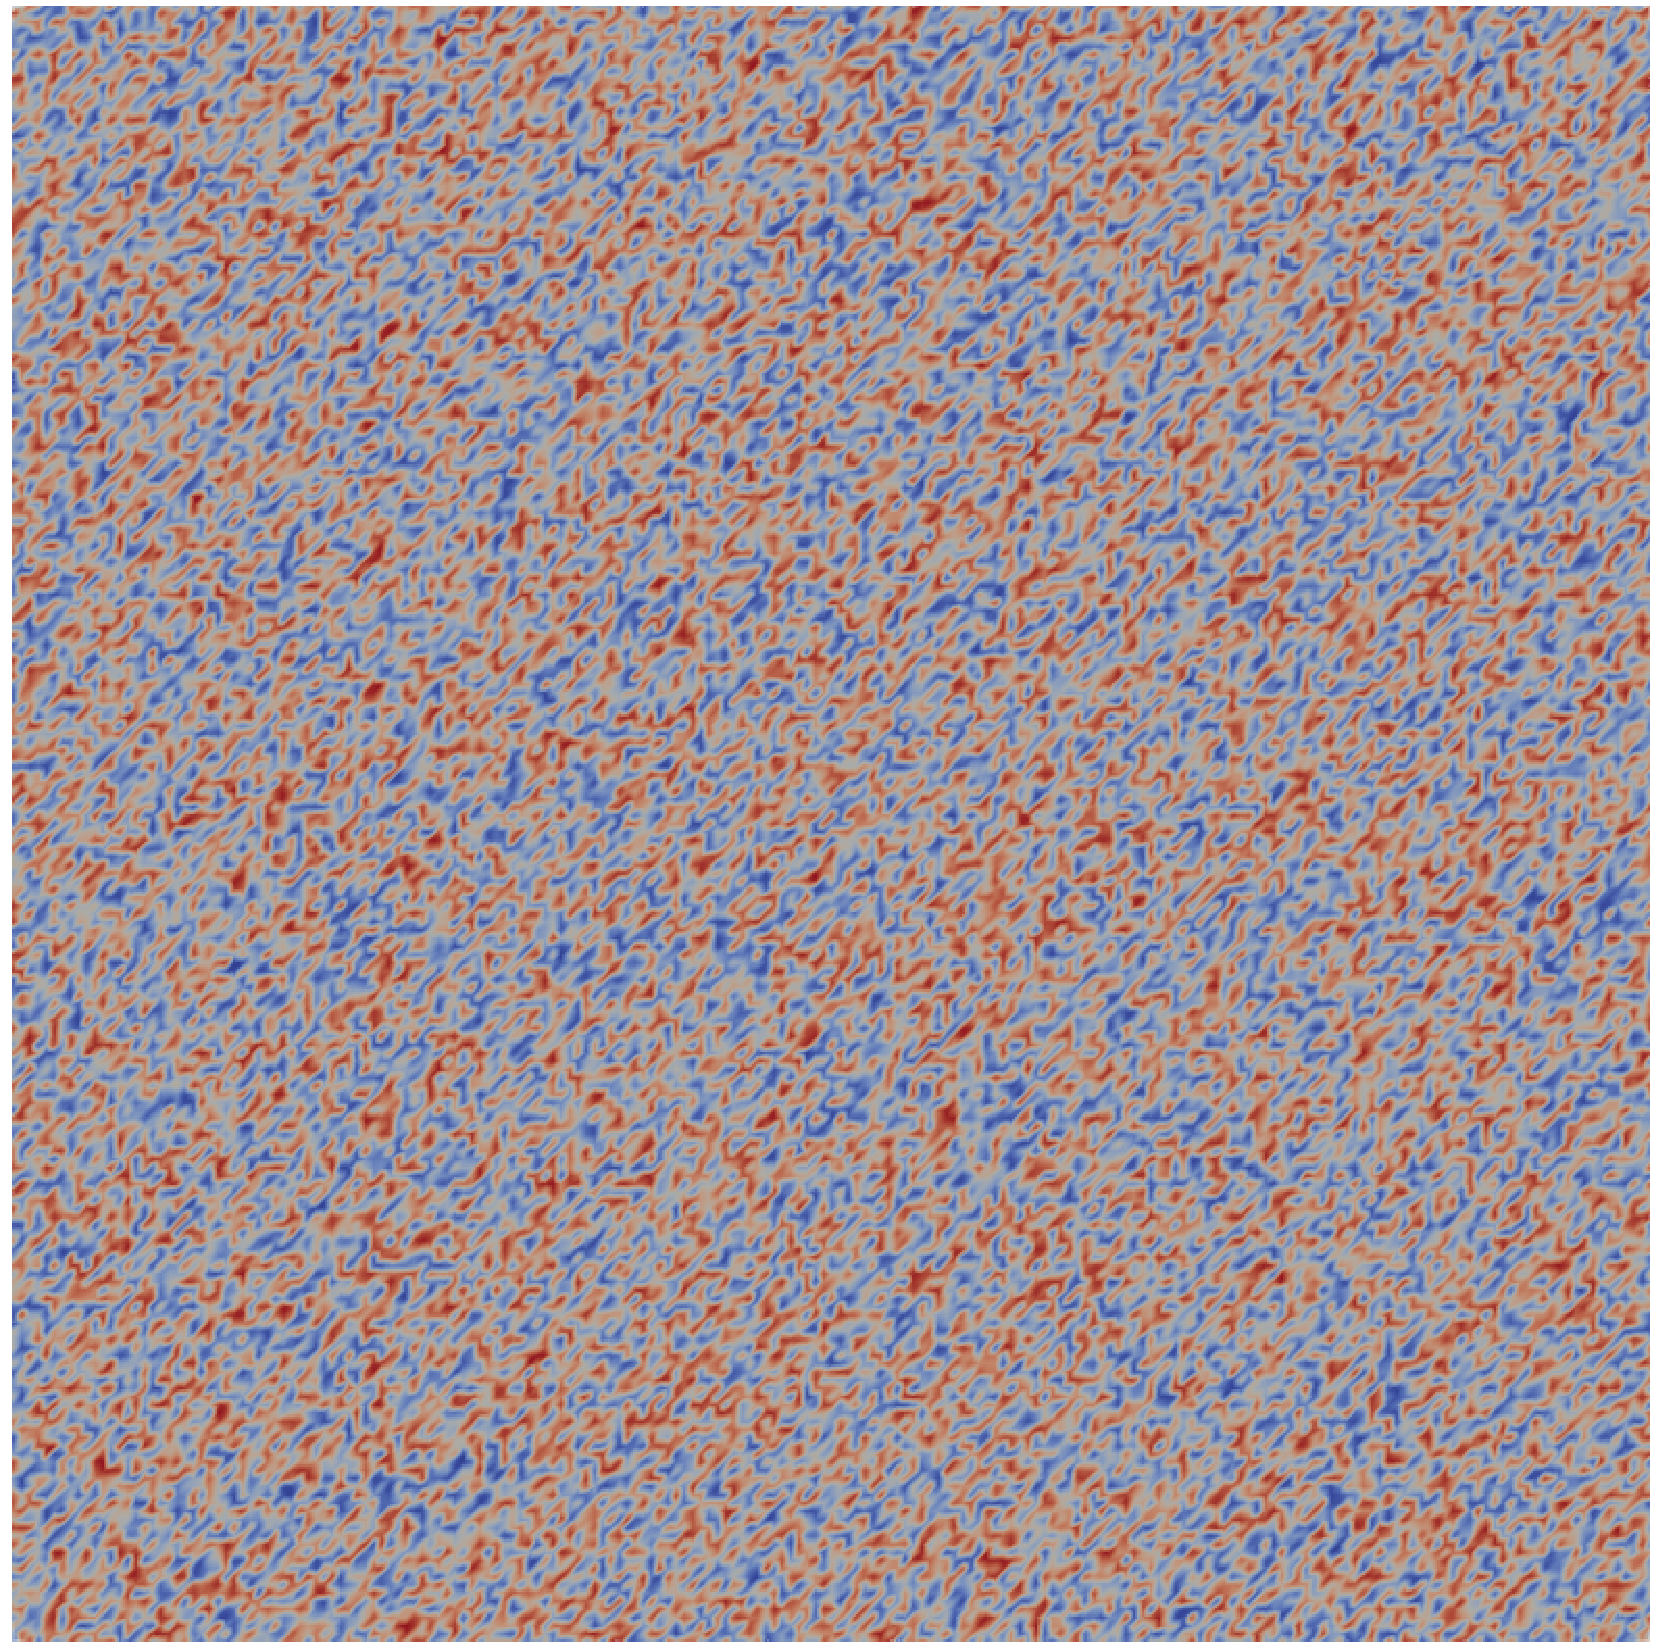
\includegraphics[width=0.95\textwidth]{Imagenes/Maxwell2D/Maxwell2D_sim/Imagenes/t_0}
        \caption{$t=0$}
    \end{subfigure}
    \begin{subfigure}[t]{0.45\textwidth}
        \centering
        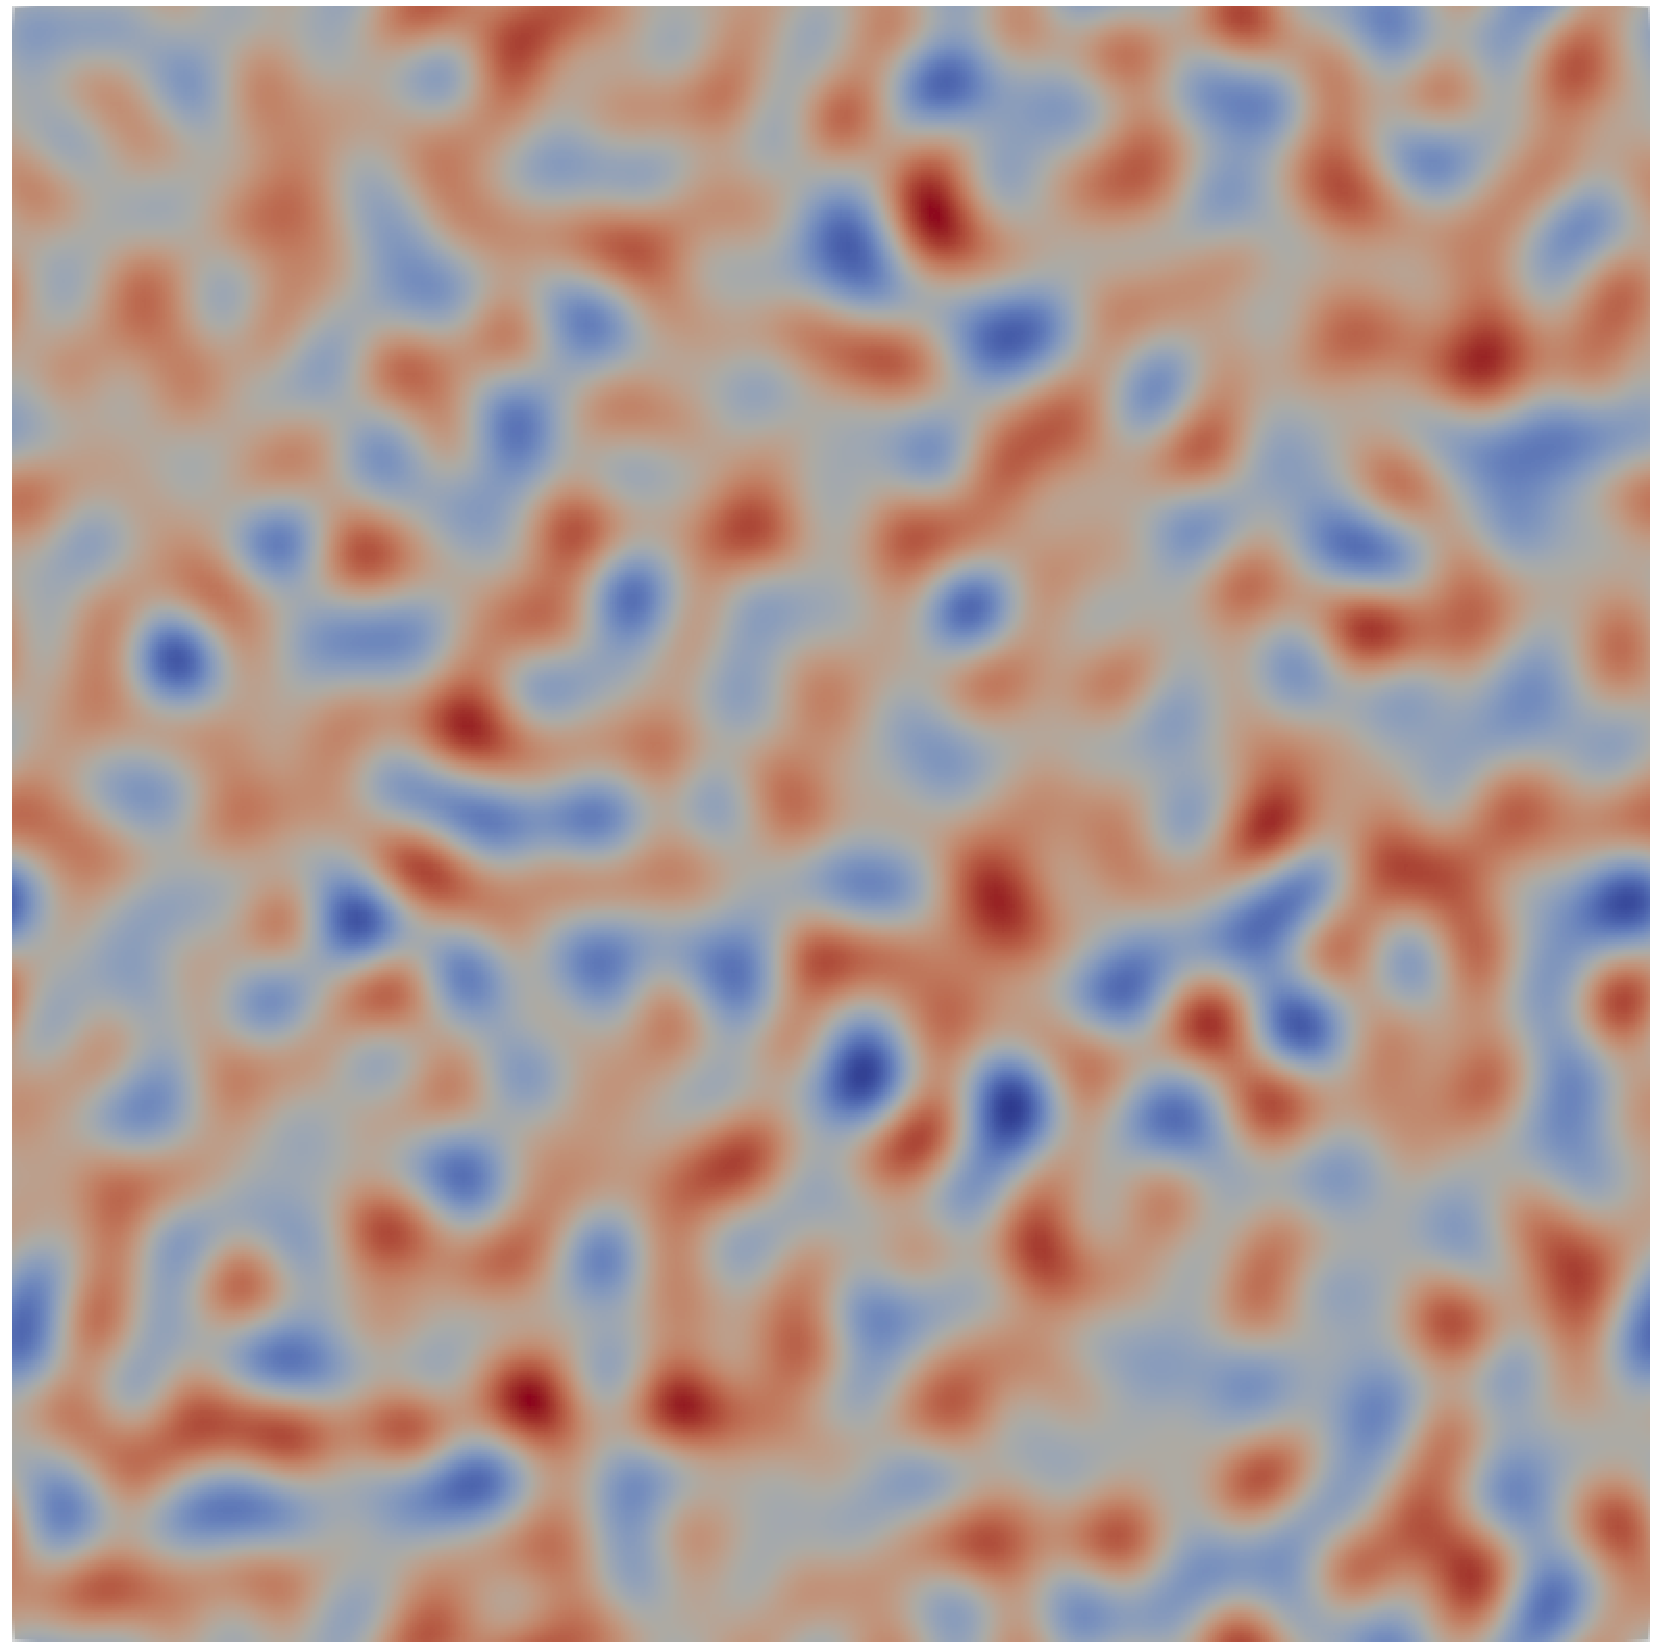
\includegraphics[width=0.95\textwidth]{Imagenes/Maxwell2D/Maxwell2D_sim/Imagenes/t_50}
        \caption{$t = 50$}
    \end{subfigure}
    \begin{subfigure}[t]{0.45\textwidth}
        \centering
        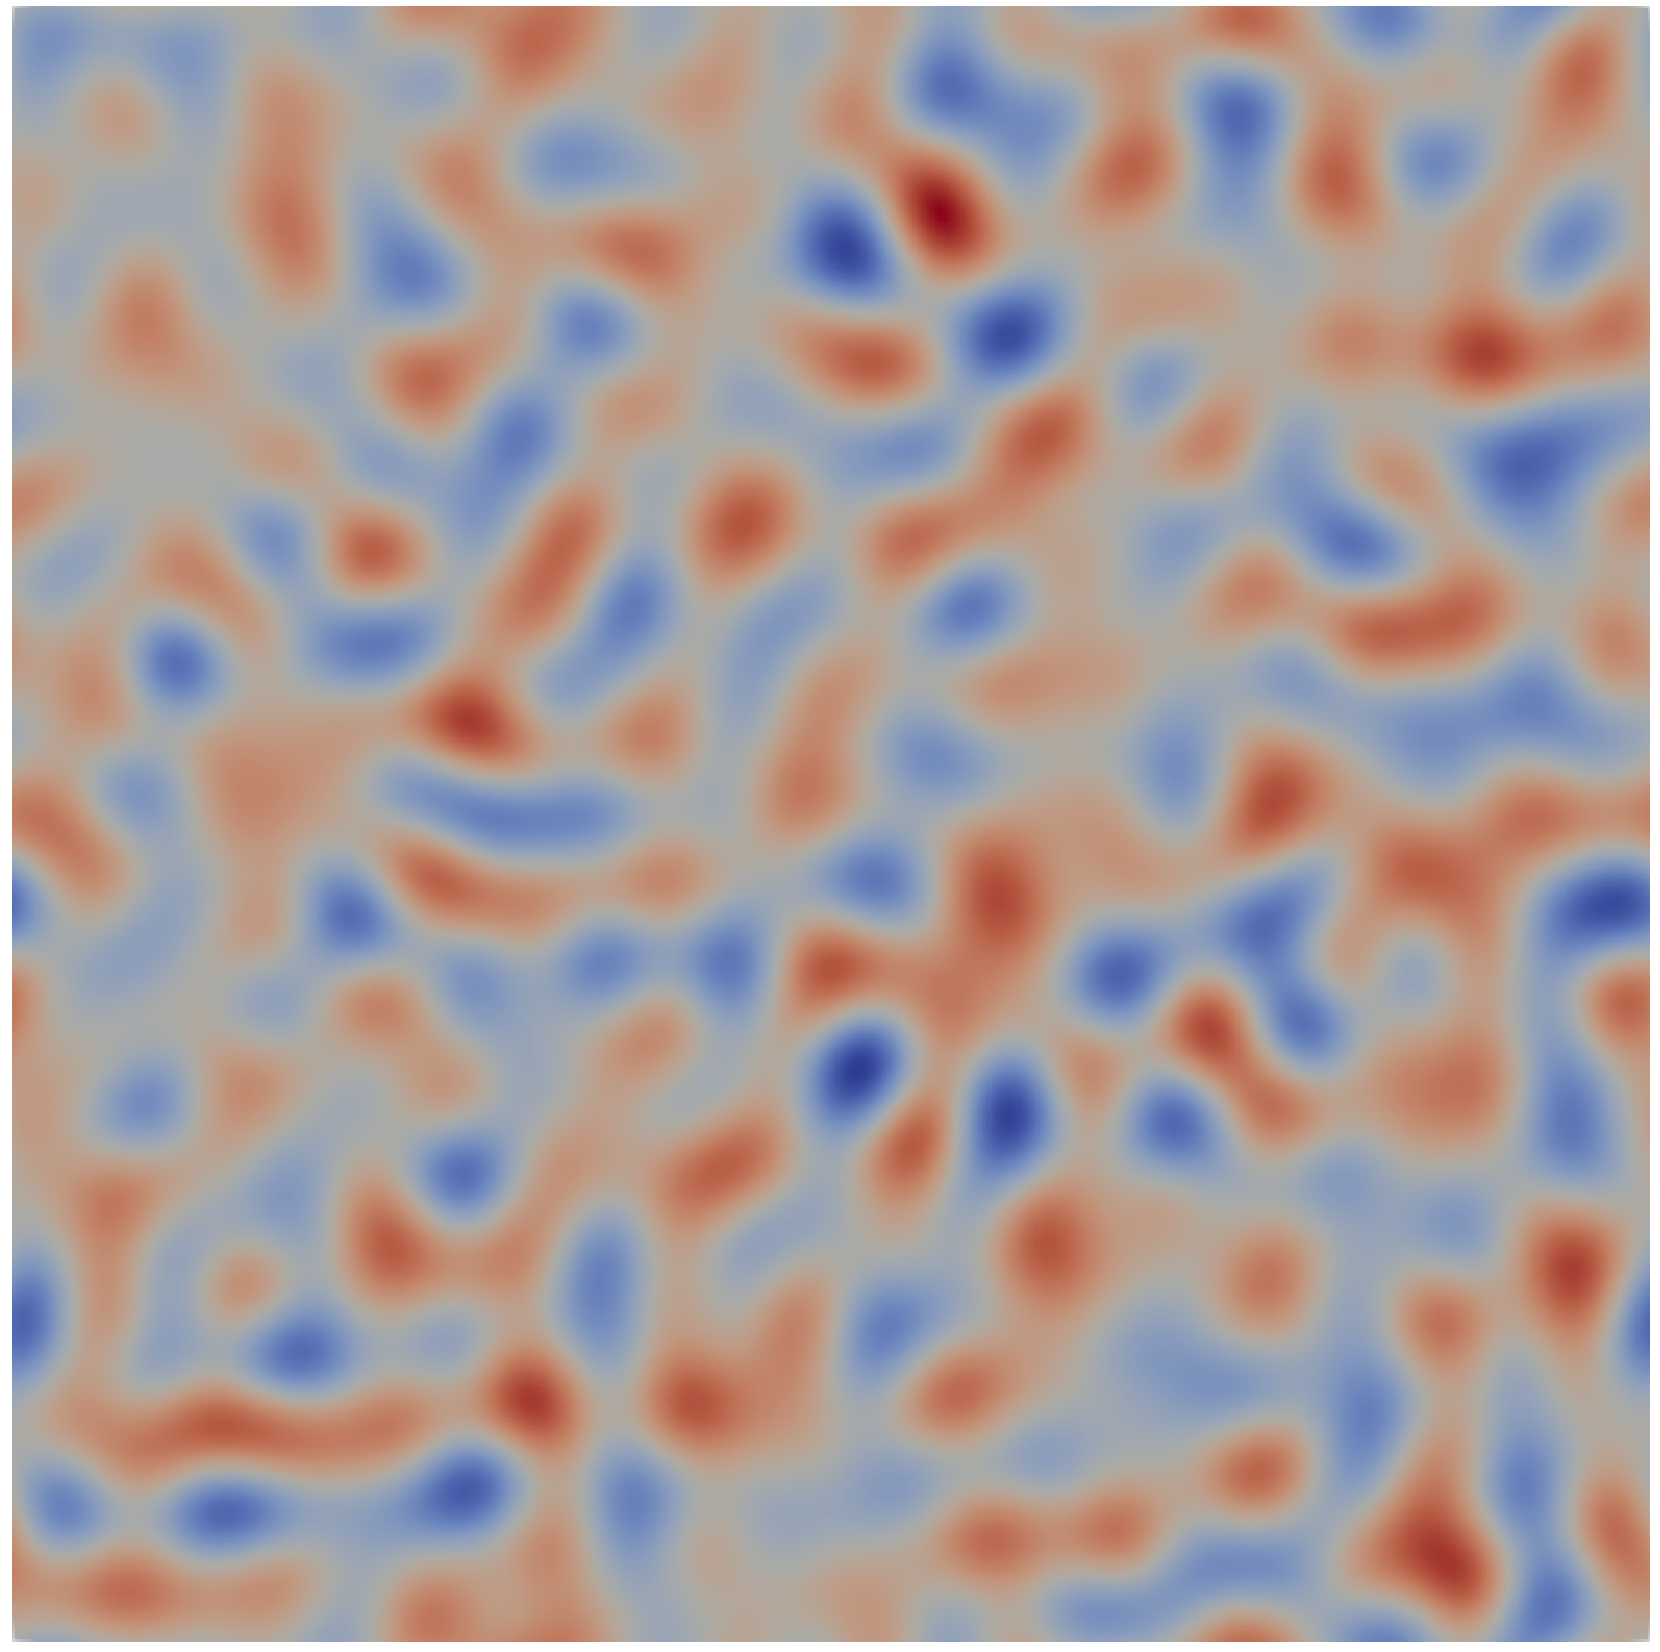
\includegraphics[width=0.95\textwidth]{Imagenes/Maxwell2D/Maxwell2D_sim/Imagenes/t_100}
        \caption{$t = 100$}
    \end{subfigure}    
    \begin{subfigure}[t]{0.45\textwidth}
        \centering
        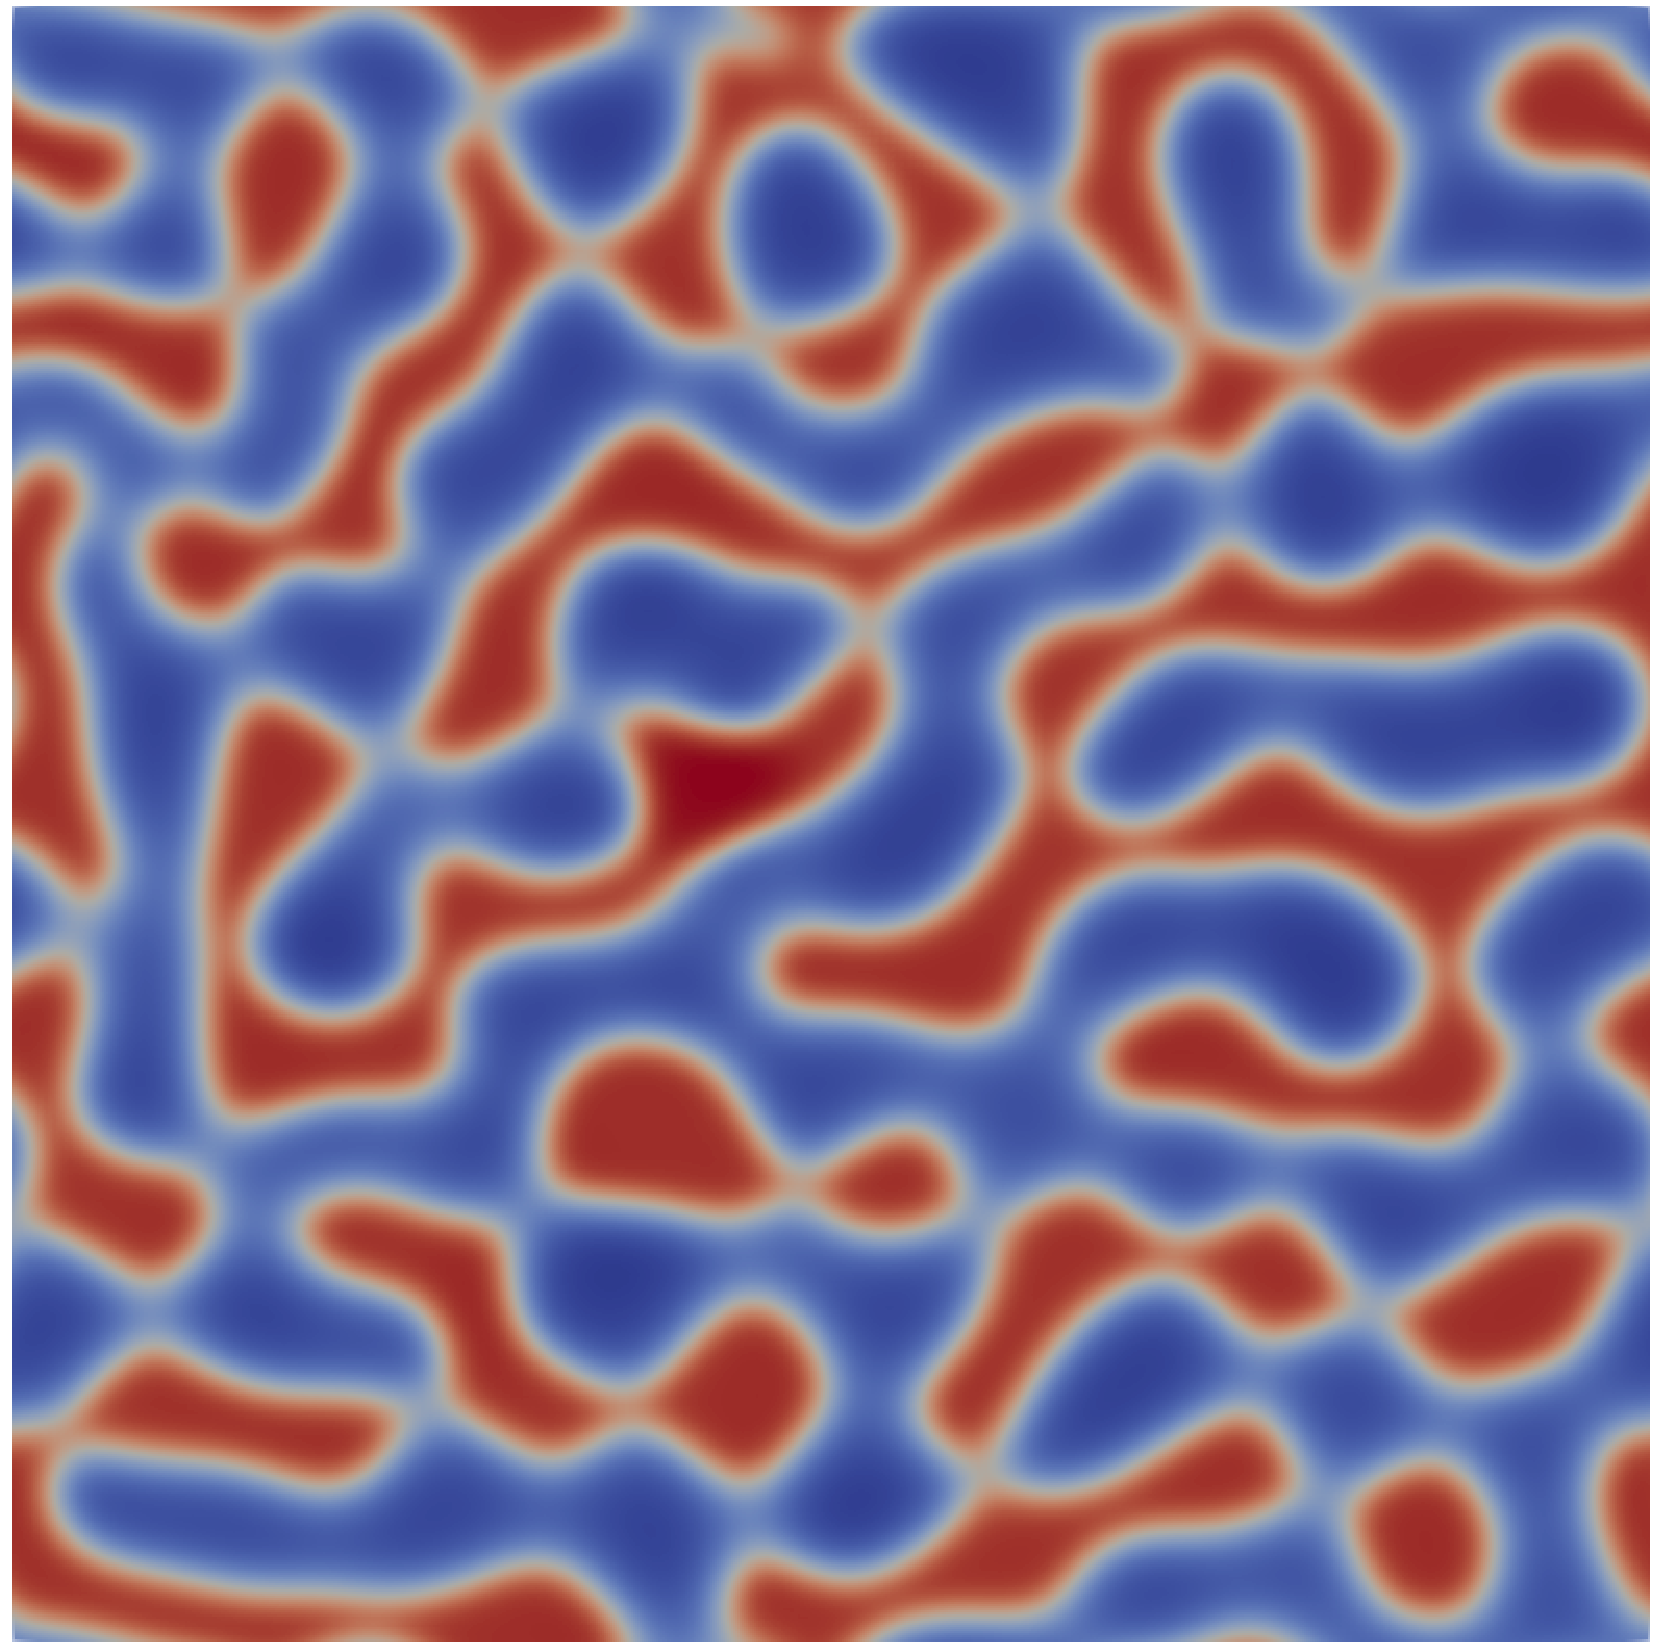
\includegraphics[width=0.95\textwidth]{Imagenes/Maxwell2D/Maxwell2D_sim/Imagenes/t_500}
        \caption{$t = 500$}
    \end{subfigure}    
    \begin{subfigure}[t]{0.45\textwidth}
        \centering
        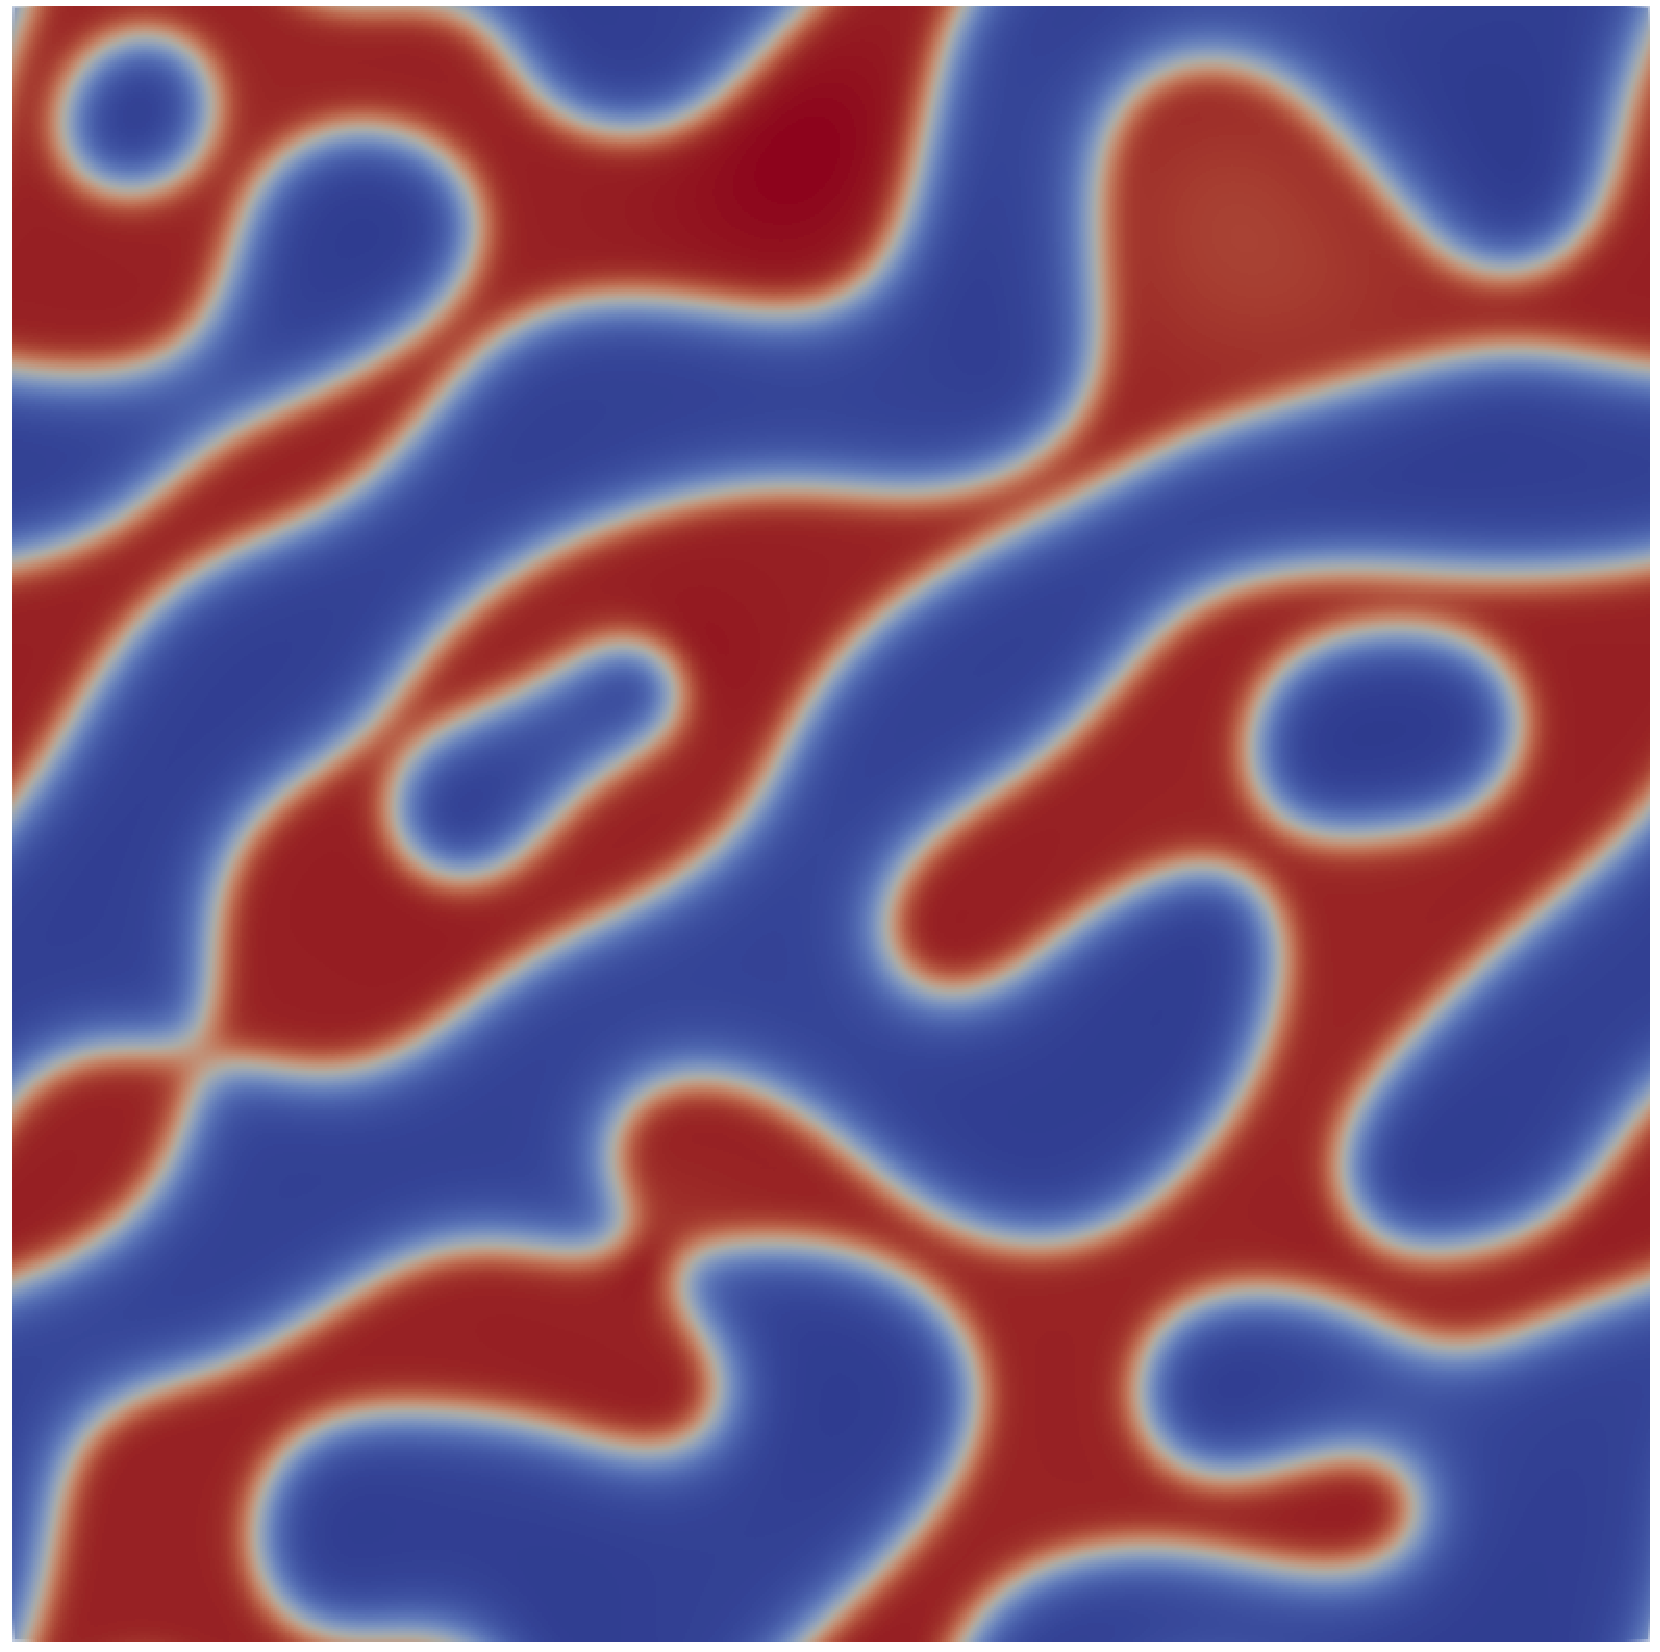
\includegraphics[width=0.95\textwidth]{Imagenes/Maxwell2D/Maxwell2D_sim/Imagenes/t_1000}
        \caption{$t = 1000$}
    \end{subfigure}
    \begin{subfigure}[t]{0.45\textwidth}
        \centering
        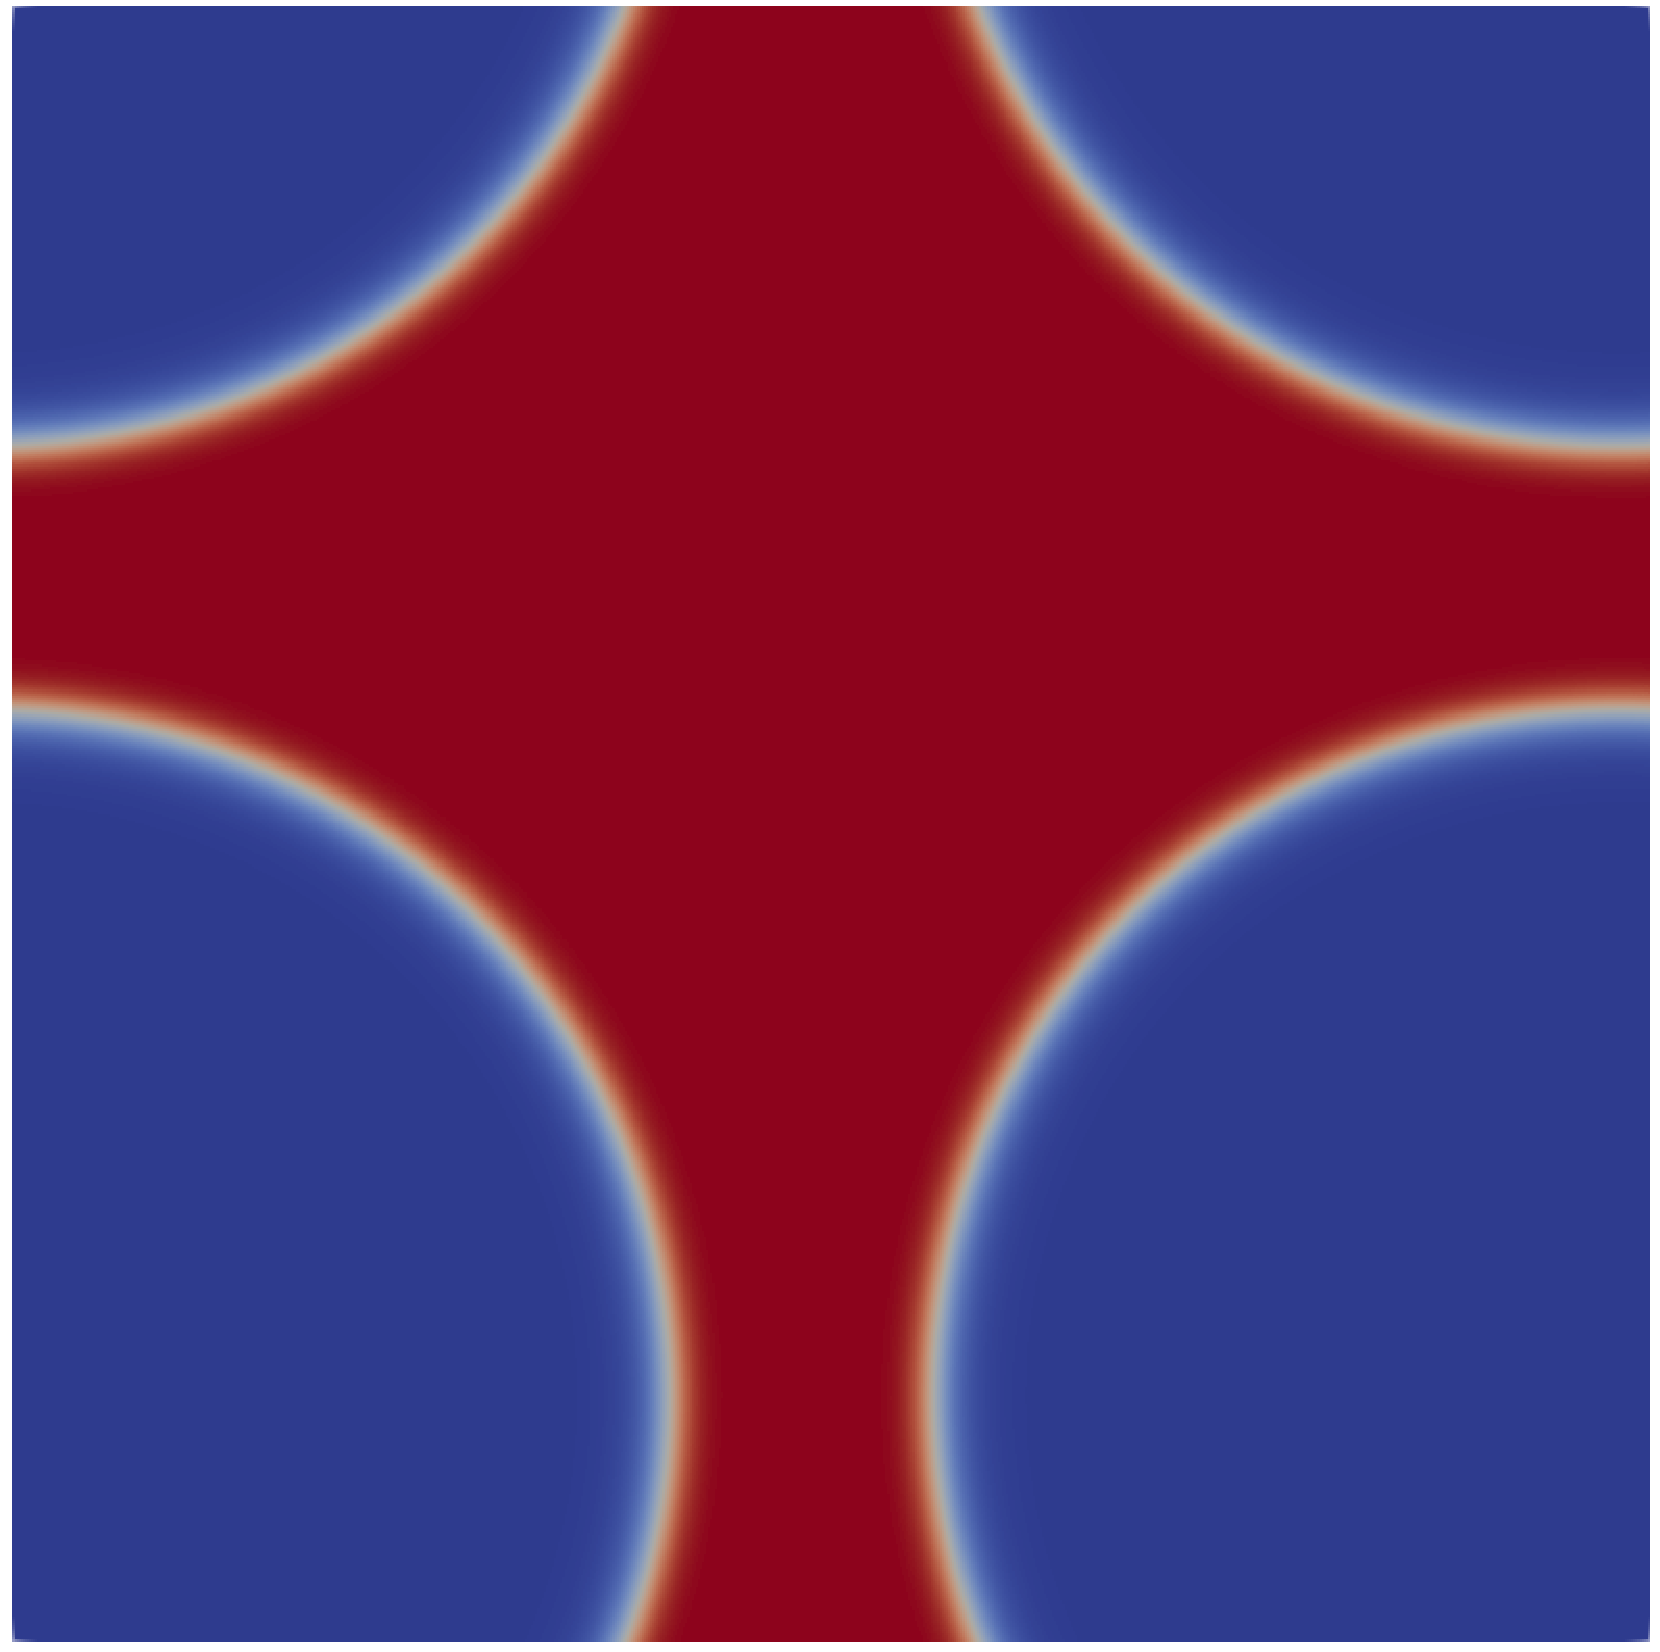
\includegraphics[width=0.95\textwidth]{Imagenes/Maxwell2D/Maxwell2D_sim/Imagenes/t_50000}
        \caption{$t = 50000$}
    \end{subfigure}        
    \caption{Evoluci\'on de una regi\'on tridimensional, peri\'odica, isot\'ermica y sin fuerzas externas, usada para verificar la regla de construcci\'on de Maxwell. La regi\'on mostrada corresponde a la fase de menor densidad.}
    \label{fig:maxwell_3d}
\end{figure}
\FloatBarrier



\section{Conclusiones}

La utilizaci\'on de ecuaciones con operador de colisi\'on MRT en la simulaci\'on del transporte de energ\'ia en flujos multif\'asicos, provee una alternativa flexible para el desarrollo de modelos t\'ermicos vinculados a los modelos isot\'ermicos de la familia \pp{}. En particular, la propuesta de \lbe{} construida sobre una conjunto de velocidades D2Q9 pudo ser extendida a grillas D3Q15, considerando una adaptaci\'on adecuada de la distribuci\'on de equilibrio, t\'ermino de fuente y elementos extra-diagonales de la matriz de relajaci\'on. De esta manera, se obtuvo una \lbe{} que permite recuperar la ecuaci\'on de energ\'ia de M\'arkus y H\'azi sin t\'erminos no deseados, con una difusividad t\'ermica recuperada que puede ajustarse con los factores de relajaci\'on o, alternativamente, con par\'ametros libres asociados a la distribuci\'on de equilibrio.

De manera similar a lo observado para la versi\'on bidimensional, el nuevo modelo es capaz de reproducir la distribuci\'on de densidad y temperatura para un fluido con \eos{} de vdW dentro de una cavidad bajo acci\'on de la cavidad. Los resultados obtenidos con este modelo, nuevamente, muestran consistencia al ser analizados empleando unidades reducidas. Por otro lado, se observ\'o que esta propuesta permite simular adecuadamente el problema de Stefan unidimensional, demostrando que es posible recuperar adecuadamente el calor latente y la difusividad t\'ermica asociados al uso arbitrario de las constantes de la \eos{} y de los par\'ametros libres de la \edf{}.